%% Select the dissertation mode on
%
% See the documentation for more information about the available class options 
% ('math', 'vertlayout', 'pdfa', ...)
% If you give option 'draft' or 'draft*', the draft mode is turned on
% NOTE if you want to generate abstracts for the publication platform, use
% the option 'abstracts'!
% The pdfa option is experimental, but give it a try -- your doc will be better archivable
%
\documentclass[dissertation,math,vertlayout,pdfa,colorlinks]{aaltoseries}

% Kludge to make sure we have utf8 input (check that this file is utf8!)
\makeatletter
\@ifpackageloaded{inputenc}{%
  \inputencoding{utf8}}{%
  \usepackage[utf8]{inputenc}}
\makeatother

% for live links. Takes the above option 'colorlinks' (use 'hidelinks' if you want them black for print).
\usepackage{hyperref} 

% Lipsum package generates quasi latin filler text
\usepackage{lipsum}
% Set the document languages used
\usepackage[english]{babel}
% more math symbols and environments if needed
\usepackage{amsmath,amssymb,amsthm} 
% after amsmath to restore bad page breaks in the middle of equations... only for those in the know
\interdisplaylinepenalty=2500 
% Adjust math line spacing
\renewcommand*{\arraystretch}{1.2} % for array/matrix environments
\setlength{\jot}{8pt} % for split environment

\usepackage{listings} % neat printing of source code
\usepackage[indentfirst=false,vskip=3mm]{quoting} % flexible quotes and quotations
% Enable the following to suppress page headers and numbers on 
% content-less left (even-numbered) pages. Fixes a bug in aaltoseries
\usepackage{emptypage}
\usepackage[nobiblatex]{xurl}


%Mathematical notations used 
\usepackage{amsmath}
\usepackage{amsfonts}
\usepackage{mathtools}
\usepackage{bm}

\newcommand{\bw}{\bm{w}}
\newcommand{\bX}{\bm{X}}
\newcommand{\by}{\bm{y}}
\newcommand{\bD}{\mathcal{D}}
\newcommand{\bF}{\mathcal{F}}
\DeclareMathOperator{\eye}{\textbf{I}}

\DeclarePairedDelimiterX{\infdivx}[2]{[}{]}{%
	#1\;\delimsize\|\;#2%
}
\DeclareMathOperator{\KLt}{KL}
\newcommand{\KL}{\KLt\infdivx}
\DeclareMathOperator{\betapdf}{Beta}
\DeclareMathOperator{\bernoullipdf}{Bernoulli}
\DeclareMathOperator{\normalpdf}{N}
\DeclareMathOperator{\gammapdf}{Gamma}
\DeclareMathOperator{\new}{new}
\DeclareMathOperator{\old}{old}
\DeclareMathOperator{\E}{\mathbb{E}}
\DeclareMathOperator{\var}{var}
\newcommand{\tp}{^{\top}}
\DeclareMathOperator*{\argmax}{arg\,max}

\usepackage{tikz}
\usetikzlibrary{arrows,decorations.pathmorphing,backgrounds,fit,positioning,shapes.symbols,chains}

\usepackage{graphicx}
%%
%% There's a HUGE number of LaTeX packages. Whatever it is you need, search for a package first before rolling your own!
%%

% This is the way you may input and separately develop your individual chapters. Write, e.g., 
%
%	%\input{Ch1}
%	%\input{Ch2}
%	\input{Ch3}
%	%\input{Ch4}
%	%\input{Ch5}
%
% ...when editing only the third chapter. Compilation with pdflatex ('pdflatex dissertation') will then only output
% a thin dissertation containing only the third chapter, but properly formatted.
%
% You may leave of the .tex extension here...
%
%    Some definitions useful in producing this sort of documentation:
\chardef\bslash=`\\ % p. 424, TeXbook
%    Normalized (nonbold, nonitalic) tt font, to avoid font
%    substitution warning messages if tt is used inside section
%    headings and other places where odd font combinations might
%    result.
\newcommand{\ntt}{\normalfont\ttfamily}
%    command name
\newcommand{\cn}[1]{{\protect\ntt\bslash#1}}
%    LaTeX package name
\newcommand{\pkg}[1]{{\protect\ntt#1}}
%    File name
\newcommand{\fn}[1]{{\protect\ntt#1}}
%    environment name
\newcommand{\env}[1]{{\protect\ntt#1}}
\hfuzz1pc % Don't bother to report overfull boxes if overage is < 1pc

%       Theorem environments

%% \theoremstyle{plain} %% This is the default
\newtheorem{thm}{Theorem}[section]
\newtheorem{cor}[thm]{Corollary}
\newtheorem{lem}[thm]{Lemma}
\newtheorem{prop}[thm]{Proposition}
\newtheorem{ax}{Axiom}

\theoremstyle{definition}
\newtheorem{defn}{Definition}[section]

\theoremstyle{remark}
\newtheorem{rem}{Remark}[section]
\newtheorem*{notation}{Notation}

%\numberwithin{equation}{section}

\newcommand{\thmref}[1]{Theorem~\ref{#1}}
\newcommand{\secref}[1]{\S\ref{#1}}
\newcommand{\lemref}[1]{Lemma~\ref{#1}}

\newcommand{\bysame}{\mbox{\rule{3em}{.4pt}}\,}

%       Math definitions

\newcommand{\A}{\mathcal{A}}
\newcommand{\BB}{\mathcal{B}}
\newcommand{\st}{\sigma}
\newcommand{\XcY}{{(X,Y)}}
\newcommand{\SX}{{S_X}}
\newcommand{\SY}{{S_Y}}
\newcommand{\SXY}{{S_{X,Y}}}
\newcommand{\SXgYy}{{S_{X|Y}(y)}}
\newcommand{\Cw}[1]{{\hat C_#1(X|Y)}}
\newcommand{\GG}{{G(X|Y)}}
\newcommand{\PY}{{P_{\mathcal{Y}}}}
\newcommand{\X}{\mathcal{X}}
\newcommand{\wt}{\widetilde}
\newcommand{\wh}{\widehat}

\DeclareMathOperator{\per}{per}
\DeclareMathOperator{\cov}{cov}
\DeclareMathOperator{\non}{non}
\DeclareMathOperator{\cf}{cf}
\DeclareMathOperator{\add}{add}
\DeclareMathOperator{\Cham}{Cham}
\DeclareMathOperator{\IM}{Im}
\DeclareMathOperator{\esssup}{ess\,sup}
\DeclareMathOperator{\meas}{meas}
\DeclareMathOperator{\seg}{seg}

%    \interval is used to provide better spacing after a [ that
%    is used as a closing delimiter.
\newcommand{\interval}[1]{\mathinner{#1}}

%    Notation for an expression evaluated at a particular condition. The
%    optional argument can be used to override automatic sizing of the
%    right vert bar, e.g. \eval[\biggr]{...}_{...}
\newcommand{\eval}[2][\right]{\relax
  \ifx#1\right\relax \left.\fi#2#1\rvert}

%    Enclose the argument in vert-bar delimiters:
\newcommand{\envert}[1]{\left\lvert#1\right\rvert}
\let\abs=\envert

%    Enclose the argument in double-vert-bar delimiters:
\newcommand{\enVert}[1]{\left\lVert#1\right\rVert}
\let\norm=\enVert



% The author of the dissertation
\author{Pedram Daee}
% The title of the thesis
\title{Probabilistic user modelling methods for improving human-in-the-loop machine learning} % This is the title of our line of work as a group.

%Comments from meeting with Sami on 15.07.2019:
% "user modelling" may not be the best term as people may perceive it as a statitstic UM. But "probabilistic user modelling" in a good context may be OK.
%  We want to have User + probabilistic in the title.
% Alternatives for user could be human-in-the-loop or user interaction or HCI or modellign of the user or interactive user modelling
% an alternative title could be to directly mention what I did: knowledge elicitation or multi source feedback. Or use these as subtitles?


%Keywords: Interactive intent modelling, User modelling, Interactive knowledge elicitation, Active elicitation of knowledge, Sequential probabilistic inference, high-dimensional prediction.
%0. Probabilistic user modelling methods for improving human-in-the-loop machine learning
%1.	Probabilistic User Modelling in Interactive Machine Learning for Prediction
%2.	Machine learning methods for user modelling for improved prediction.
%3.	Interactive user/expert modelling for improved prediction 
%4.	Machine Learning Methods for Improved Prediction through Probabilistic User Modelling
%5.	Improved Prediction through Interactive Probabilistic User Modelling
%6.	Probabilistic user modelling methods for improving human-in-the-loop machine learning.

%Other comments: I do not like knowledge elicitation since it seems like a term that may become obsolete through time

\begin{document}

%% The abstract of the dissertation in English
% Use this command!
%\draftabstract{\lipsum[1-2]}%
%\draftabstract[english]{\hspace{-2pt} My abstract in English}
% Let's add another one in Finnish
%\draftabstract[finnish]{\hspace{-2pt} En puhu suomea1

%}%


% And yet another one in Swedish
%\draftabstract[swedish]{\lipsum[7-9]}
%%---------------------

%% The abstract of the dissertation in English
% Use this command!
%\begin{abstract}\lipsum[1-3]\end{abstract}%
% Let's add another one in Finnish

\begin{abstract}[english]
	
\noindent Ongoing title: \\
\textbf{Probabilistic user modelling methods for improving human-in-the-loop machine learning}
%\noindent\textbf{2. Probabilistic user modelling methods for improving human-in-the-loop machine learning}
%\noindent\textbf{3. Interactive user modelling for human-in-the-loop machine learning} % NOTE: Interactive and in-the-loop are a bit redundant
%Sami's comment about the title: All these are OK but still broad. Many people in the group could have the same title.	
\\
\\
In many machine learning applications and in particular those with only few training data, human involvement in the form of data provider or expert of the task is crucial. However, human interaction with a machine learning model is constrained by (i) the interaction channels, i.e., how human knowledge can be applied in the model, and (ii) the interaction budget, i.e., how much the user is willing to interact with the model. This thesis proposes new methods to improve theses constrains in human-in-the-loop machine learning. The core idea of the thesis is to jointly model the available data with a model of the human user, i.e., the user model, in a unified probabilistic model and then perform sequential probabilistic inference on the joint model to design improved interaction. The thesis contributes on two types of prediction tasks.
\\\\
The first task is the expert knowledge elicitation for high-dimensional prediction. Experts in the fields usually have information beyond training data which can help to improve the prediction performance. The thesis contributes by proposing user models, as likelihood functions, to directly connect expert knowledge about the relevance of parameters to a linear model responsible for prediction. The user model can account for complex user behaviour such as the fact that users may update their knowledge during the interaction. %, which allows to gain more information from interaction. 
Furthermore, sequential experimental design on the joint model is employed to query the most informative expert knowledge earlier. 
\\\\
The second task is the personalized recommender system that tries to predict the most relevant item for a user with few interactions. The interaction is based on user relevance feedback on the recommendations. The thesis contribute by proposing user models that are able to receive and integrate feedback on multiple domains and sources by providing a joint probabilistic model connecting all feedback types. Sequential inference on the joint model, using Thompson sampling, was employed to find the targeted recommendation with minimum interaction.    
\\\\
Simulated experiments and user studies in both tasks demonstrate improved prediction performance only after few interactions with the users.
\\\\\\\\
\textbf{Keywords} Interactive machine learning, Bayesian inference, probabilistic user modelling
%However, the  amount of interactions that a human user can have with a model is usually limited due to the user's reluctance or the time and workload constrains. This thesis studies approaches to improve human-in-the-loop machine learning with minimal interaction. The core idea of the thesis is to jointly model the human user with the available data in a unified probabilistic model and then perform sequential probabilistic inference on the joint model to design improved interaction. The thesis contributes on two types of tasks.


%The first contribution is to 


%The proposed feedback models provide an intuitive and effortless way for the user to influence the prediction model without caring about the mathematical complications of the data model. The feedback models are a communication channel for transferring expert knowledge to the unknown parameters of the models.
	


%\begin{itemize}
%    \item Human and intelligent systems are increasingly interacting with each other. 
%    \item Add one sentence why it is a hard problem, then add another sentence that “and that is why we …..” to connect to your contribution.
%    \item gist: joint model of human and data through active learning, experimental design on a budget %Sami
%\end{itemize}



%TODO: Need to define user modelling to some extent here. by user models, i.e., what the ML system is able to think of the user.
% Go into the gist and why it is different and what is done immediately.  Sami thinks that intent modelling in IR is not prediction, but we model and solved it as a prediction problem. Maybe have “relevance of variables” as a keyword since this may be what I am doing. Regarding the title, keep the spirit but focus more. E.g., “human intent modelling for eliciting importance of variables” (knowledge elicitation?).
\end{abstract}

%1. What is the bigger picture?
%2. Dissertation purpose
%3. Research method
%4. Key results
%5. Practical Implications

%Typically 3 paragraphs: 1. the introduction of the challenge problem, 2. thesis, 3. contribution

 
%\begin{abstract}%[finnish]
%En puhu suomea.
%\end{abstract}


% And yet another one in Swedish
%\begin{abstract}[swedish]\lipsum[7-9]\end{abstract}


%% Preface
\begin{preface}[Espoo]
%Acknowledgements: 

% ML17:
% Grants 295503, 294238, and 284642), 
%IUI18:
% Grants 295503, 294238, and 284642),  
%Bio 19:
%grants 295503, 294238, 284642, 305780, 286607 and 294015],
%Jasist:
% We thank Mats Sjöberg, Antti Kangasrääsiö, for their hard work in imple- menting the system and running experimental studies.


This thesis is the result of research conducted in the Probabilistic Machine Learning (PML) group at the Department of Computer Science at Aalto University. I was fortunate to receive financial support for the thesis from the Academy of Finland (Finnish Center of Excellence in Computational Inference Research COIN, Grants 295503, 294238, and 284642), Re:Know funded by TEKES, the European Commission (MindSee FP7-ICT; Grant Agreement \#611570), and the Nokia foundation. 

I wish to express my sincere appreciation to Samuel Kaski for the guidance and invaluable insight into research, for all the honest, sometimes harsh, but to the point comments, and for being an example of excellent management skills. I wish to also thank him for his support and encouragement to travel to international scientific gatherings which allowed me to gain invaluable experience both in research and in life.

I had great pleasure of working with all my co-authors who contributed in the publications included in this thesis: Joel Pyykk\"o, Dorota G\l{}owacka, Tomi Peltola, Marta Soare, Iiris Sundin, Luana Micallef, Homayun Afrabandpey, Muntasir Mamun Majumder, Chen He, Baris Serim, Aki Havulinna, Caroline Heckman, Pekka Marttinen, Aki Vehtari, Oswald Barral, Markus Wenzel, Tuukka Ruotsalo, Patrik Pluchino, Jonathan Freeman, Luciano Gamberini, Benjamin Blankertz, and Giulio Jacucci. % and also co-authors in the publications that are not part of the thesis: Mustafa Mert \c{C}elikok, Fabio Colella, Jussi Jokinen, and Antti Oulasvirta. 
In particular, I would like to express my deepest appreciation to Tomi Peltola for his invaluable contributions and for being a role model for doing rigorous science. %manzur ine ke be kar nega kone na nazare khodehs

I am also grateful to the former and current members of PML group for all the scientific discussions, frequent fussball games, and other fun activities. Just to mention few, I would like to thank Marta Soare, Andrej Gisbrecht, Jussi Gillberg, Eemeli Leppäaho, Antti Kangasrääsiö, Muhammad Ammad-ud-din, Iiris Sundin, Mustafa Mert \c{C}elikok, and Fabio Colella. Particular tribute to my friend and fussball teammate Homayun Afrabandpey who was always available for in depth discussions and challenging games. 

Special thanks to XXX and XXX for accepting to be the pre-examiners of this thesis. ... %. I gratefully acknowledge the assistance of
and Samuel Kaski, XXX, and XXX for proofreading the thesis. 

I would like to thank Ari Vepsäläinen and Katrina Nordström for their kindness and hospitality from the first day I moved to Finland and all my friends, in particular Navid Khajehzadeh, Hanieh Poostchi, Kourosh Latifi, Parvin Pashang, Saeed Mirzaeifar who made the new life to feel as joyful as home. %helped me adapt and 

My deepest gratitude to my parents, Kazem and Sima, and two brothers, Poria and Pejman, in Iran who unconditionally supported me through every step of my life. Last but not least, I would like to thank my wife, Shaghayegh, for her continued love and support and for being my best friend in life.

\end{preface}

%% Table of contents of the dissertation
\clearpage
\tableofcontents

% To be defined before generating list of publications. Leave off if no acknowledgement
%\languagecheck{the Institute of Language Checks}

%% This is for article dissertations. Remove if you write a monograph dissertation.
% The actual publications are entered manually one by one as shown further down:
% use \addpublication, \addcontribution, \adderrata, and addpublicationpdf.
% The last adds the actual article, the other three enter related information
% that will be collected in lists -- like this one.
\listofpublications

%% Add lists of figures and tables as you usually do (\listoffigures, \listoftables)

%%%%%%%%%%%%%%%%%%%%%%% do I want to have the followings? 
%\listoffigures
%\listoftables

%\abbreviations
%\begin{description}
%\item[PDF] Probability Density Function
%\end{description}

%\symbols
%\begin{description}
%\item[$p(\theta \mid y)$] Conditional distribution
%\end{description}


%% The main matter, one can obviously use \input or \include
\chapter{Introduction}
%Comments from meeting with Sami on 15.07.2019:
% I need to tie to non-ML related works somewhere in the paper. This can include HCI related works or knowledge elicitation or multi agent? I need to either list them here and give a short description or put them inside the next two chapters. In any case, I need to refer back to these in the Discussion section and mention how we improved the fields (and how we benefited from these).

\section{Motivation}

Whether it is a user searching for information in a search system or a doctor working with a cancer diagnostic system, humans and machine learning systems are increasingly interacting with each other \cite{amershi2014power}. This thesis studies the family of human-machine interaction problems where the goal of the interaction is to solve a prediction problem, i.e., predicting a response variable corresponding to an input. Such problems can include predicting how much a user likes items in a personalized search activity, or medical prediction about the response of a cancer drug. An important common factor in these scenarios is that the number of labeled data (known as training data) that the machine can use to make predictions, is less than the dimension of the search space. This is known as the ``small $n$, large $p$'' problem, where $n$ refers to the number of available labeled data and $p$ the dimension of the problem determined by, for example, the number of variables. These types of problems result in ill-posed statistical learning since there are limits in how low in sample size statistical methods can go \cite{Donoho2009observed}. 

%The aim of this thesis is to improve this interaction by incorporating a probabilistic model of the human user in the system they are interacting with. 
 

%To improve usability and usefulness of such human--computer interaction, user modelling enables the machine to have a better understanding of the user's interaction \cite{user_modelling_2001}. 

%User modelling provides the machine with a model for explaining user inputs to the system to improve usability and usefulness of such human--computer interaction \cite{user_modelling_2001}. explaining the allows the machine to understand how 

There are different ways to handle the limited labeled data challenge. The most direct solution is to provide more labeled data for the model. However, this can be costly (e.g., testing the drug response on a new patient in the drug response prediction task) or even impractical due to the nature of the data provider (e.g., reluctance of users to provide many feedbacks about their interest in personalized search systems). An alternative direction is to restrict the model family to a simpler family of solutions (for example by assuming linearity and/or sparsity \cite{lasso2011}) to prevent the model from overfitting to the few available labeled data. 

A less explored direction for tackling the limited data challenge in human-in-the-loop systems, is to make prior assumptions about how user interaction with the system is generated and to exploit this knowledge to extract more information from the limited interaction. In other words, the machine can maintain a model of the user to better explain the user interactions and to exploit it to optimize the interaction. In this thesis, we refer to machine's model of the user as the user model (see \cite{user_modelling_2001} for a broader definition of user modelling in the context of human-computer interaction). The thesis focuses on user modelling in two general types of applications:

\paragraph{Interactive intent modelling} is the task of learning the hidden intent of a user based on a sequence of interactions \cite{ruotsalo2015interactive}. For example in personalized recommender systems, the hidden intent can be the user's interest over all items. Interaction is done through a sequence of iteration of recommendation of items and observing user feedbacks to them. The machine learning task here is to predict the user intent and to recommend the high relevant items as fast as possible. The main challenge is that the users are usually reluctant to engage with the system for a long time. %Therefore, the model needs to carefully select the items to be recommended to the user.

\paragraph{Knowledge elicitation} is the task of extracting expert knowledge about a prediction model with the goal to improve the prediction performance. For example, in drug response prediction task, there are usually few training data available, but experts in the field can have information beyond the training data that potentially can help to improve the performance. Prior elicitation techniques are classical methods to quantify experts' knowledge through interaction with statisticians who design the model \cite{OHagan06}. We are interested to remove the statisticians from the loop and directly collect the expert knowledge in the model. The challenge here is to design a communication channel between the experts and the prediction model and to efficiently extract the most gainful information.   

In both of the mentioned applications, the model needs to design the interaction in a way to achieve the goal with as few interactions as possible.  


%In particular user modelling in machine learning defines what types of interactions the user can have with the machine and how this interaction can be designed to achieve the interaction goal \cite{user_modelling_2001}.


%In its simplest form, the user model can explain the user inputs to the system for the machine or it can help the machine to provide more useful recommendation for the user. 
%This approach is known as user modelling in human--computer interaction (see for example \cite{user_modelling_2001}) and it broadly studies ways to improve usability and usefulness of human--computer collaboration.

 
\section{Research questions and contributions}


This thesis investigates methods to tackle the limited user interaction challenge in interactive machine learning for prediction. %The thesis focuses on scenarios where there are few labeled data available compared to the dimension of the problem, or when a human user is provider of the labeled data. 
The core idea of the thesis is to jointly model the human user, as a probabilistic user model, with the data in a unified probabilistic model and then perform sequential probabilistic inference on the joint model to design improved interaction.  The thesis focuses on the following research questions derived from the core idea and tasks mentioned above:\\

%\noindent \textbf{RQ1 --} \textit{Can we exploit new sources of interaction as additional learning signals from a human user to improve interactive intent modelling?}
\noindent \textbf{RQ1 --} \textit{Can we facilitate interactive intent modelling by adding new interaction domains?}

Publications I and V contribute to this research question by proposing models to incorporate new types of user feedback to amend the limited feedback in interactive intent modelling. The focused task is a document search scenario where a user needs to sequentially provide relevance feedback to suggested keywords in order to find the targeted document. %This is modelled as a multi-armed bandit problem with the goal of finding the most relevant document with minimum interaction. 
In particular, Publication I couples user relevance feedback on both documents and keywords by assuming a shared underlying latent intent model connected through a probabilistic model of the relationship between keywords and documents. The keyword and document recommendation is then done by performing sequential inference on the intent with the goal of finding the most relevant document with minimum interaction.
%Thompson sampling on the posterior of the latent intent was used to recommend new documents and keywords in each iteration. 
Publication V investigates the use of implicit relevance feedback from neurophysiology signals for effortless information seeking. The work contributes by demonstrating how to integrate this inherently noisy and implicit feedback source with scarce explicit interaction. A model for controlling the accuracy of the feedback given its nature (implicit or explicit) was introduced. 
Similar sequential inference to Publication I was used for recommendation. 
%Similar to Publication I, Thompson sampling was used to control the exploration and exploitation balance of the recommendations. 
Both publications were evaluated by user studies in realistic information seeking tasks. 


%\noindent \textbf{RQ2 --} \textit{Can expert knowledge about high-dimensional data models be elicited to improve the prediction performance?}
\noindent \textbf{RQ2 --} \textit{Can we improve prediction performance by directly extracting expert knowledge about the model?}

Publications II and III contribute by proposing a framework to directly connect the expert to the model. Publication II models knowledge elicitation as a probabilistic inference process, where the user knowledge is sequentially queried to improve predictions on a ``small $n$, large $p$'' problem.  %In particular, sparse linear regression is considered as the data model with access to only few high-dimensional training data. 
It is assumed that the experts have knowledge about the importance of variables, or of values of the regression coefficients and can provide this information to the model if queried. The work contributes by an algorithm and computational approximation for fast and efficient interaction, which sequentially identifies the most informative queries to ask from the expert. Publication III builds on Publication II by adding user knowledge about direction of relevance of variables and applying the model in an important application of precision medicine to predict the effects of different treatments using high-dimensional genomic measurements. Both publications were evaluated by extensive simulations and user studies. 
Source codes for methods presented in Publications II and III, and user study data from Publication II are available at \\ \texttt{https://github.com/HIIT/knowledge-elicitation-for-linear-regression} and \\ \texttt{https://github.com/AaltoPML/knowledge-elicitation-for-precision-medicine}.




%\noindent \textbf{RQ3 --} \textit{Is it enough to incorporate human knowledge directly in the data model as explained in RQ2, or could it be beneficial to account for rational knowledge updates that humans may undergo during the interaction?}
%\noindent \textbf{RQ3 --} \textit{Is it sufficient to directly incorporate extracted human knowledge in the model as in RQ2, or could it be beneficial to account for rational knowledge updates that humans may undergo during the interaction?}
%\noindent \textbf{RQ3 --} \textit{Could it be beneficial to have a user model that models the experts as active agents that may update their knowledge during knowledge elicitation?}

\noindent \textbf{RQ3 --} \textit{Is it beneficial to model the expert as an active agent that updates its knowledge during knowledge elicitation?}

The user models in RQ2 considers the expert as a passive data source that is not influenced by the interaction. Publication IV contributes to this research question by modelling the human expert as a rational agent that updates its knowledge about the underlying prediction task during the interaction. In particular, training data or its statistics are commonly revealed (for example through visualizations) to the user during knowledge elicitation. The elicited knowledge from the user may then be, to some extent, dependent to the knowledge coming from the training data. This redundant knowledge can  result in overfitting since the model may not account for the dependencies between training data and user feedback. We propose a user modelling methodology that assumes that the observed user feedback is an outcome of the user's rational knowledge update. The user model can then perform the inverse of the update to extract user's tacit knowledge and then update the model. The proposed user modelling idea was evaluated in a user study. 
Source code and user study data are available at \texttt{https://github.com/HIIT/human-overfitting-in-IML}.

\section{Organization of the thesis}

The thesis is organized as follows. Chapter two provides an overview of probabilistic modelling and introduces our approach of modelling the user and data as a joint probabilistic model. Chapter three investigates the design of interactions and reviews different utility functions for selecting the most informative query to be asked from the user. The fourth chapter revisits the research questions and summarizes Publications I-IV. The thesis concludes with discussions and suggestions for future directions for probabilistic user modelling.



\chapter{Probabilistic modelling of data and user} \label{prob_model_data_user}


This chapter provides a brief introduction to probabilistic modelling as the main statistical framework that is used through the thesis. After some preliminaries,  Section \ref{prob_model_data} reviews the type of linear models that are used in Publications I-V for prediction. Section \ref{prob_model_user} introduces different types of user interaction with the linear model and explains how user knowledge about the model can be incorporated as observational feedback. The computational solutions for Bayesian inference are reviewed in \ref{posteriro_inf}. %Finally, the key components for modelling observational data and user feedback as a joint probabilistic model is introduced in Section \ref{key_comp}.

\section{Preliminaries}
The core idea of probabilistic modelling is to describe all unobserved parameters and observed data as random variables from probability distributions. The unobserved parameters include the unknown quantity of interest or other parameters that affect the data or the quantity of interest. Bayesian inference provides a powerful framework to fit the described probabilistic model to observational data \cite{Gelman2013}. A core feature of Bayesian inference is that it provides probability distributions as the solution, compared to providing just a value outcome. % to deterministic methods which provide a single outcome.
This uncertainty quantification is of high interest in cases where few observational data are available or when the data acquisition scheme is controlled by the model. Both of these constrains are prominently present in the focused tasks of this thesis.

The thesis follows the notation of \cite{Gelman2013} and uses $p(.)$ to denote a probability distribution and $p(.\mid.)$ a conditional distribution. Consider the case where there is a set of observations $\bD= \{y_1,\ldots,y_n\}$ that are generated from a model with an unobserved parameter of interest $\theta$. The observational model for an observation $y$ describes the conditional density of $y$ given the parameter $\theta$ and is denoted as $y \sim p(y \mid \theta)$. It is usually assumed that the observations are conditionally independent given $\theta$, enabling us to write the model for all observations as $p(\bD \mid \theta) =  \prod_{i=1}^{n} p(y_i \mid \theta)$. The observational model is called the likelihood function if perceived as a function of $\theta$ with fixed observation $y$. One of the core tasks in statistical inference is to estimate the parameter of interest $\theta$ based on observations $\bD$. % and the likelihood assumption. 
Bayesian inference answers this question by computing the conditional distribution of $\theta$ given $\bD$ following the Bayes rule


\begin{equation}\label{Eq:Bayes}
p(\theta \mid \bD) = \frac{p(\bD \mid \theta)p(\theta)}{p(\bD)},
\end{equation}  

\noindent where $p(\theta)$ represents the prior belief about $\theta$ and $p(\bD)$ is called the marginal likelihood and acts as a normalization factor as it does not depend on $\theta$. The marginal likelihood can be computed using the marginalization rule, i.e., $p(\bD)= \int_{\theta} p(\bD, \theta)d\theta= \int_{\theta} p(\bD \mid \theta)p(\theta) d\theta$ \footnote{The integral turns to summation for discrete $\theta$.}. The conditional distribution $p(\theta \mid \bD)$ is called the posterior and it expresses the uncertainty surrounding the true value of $\theta$, after updating the prior assumptions about $\theta$ (represented by $p(\theta)$) with the knowledge coming from the observations (represented by $p(\bD \mid \theta)$).  

In many cases, we may be more interested to make a prediction about an unknown observable data point $\tilde{y}$ rather than the parameter $\theta$. Bayesian inference allows us to compute the conditional distribution of this unknown observable data given the observed data points by averaging over the posterior: 

\begin{equation}
p(\tilde{y} \mid\bD ) = \int_{\theta} p(\tilde{y}  \mid \theta)p(\theta \mid \bD)d\theta. 
\end{equation}

\noindent The conditional distribution $p(\tilde{y} \mid \bD)$ is known as the posterior predictive distribution and represents the uncertainty about a potential new observation. An example usage of this distribution could be when we want to make predictions about the test data. Since test data are unobserved, we can use posterior predictive distribution as our best guess. However, in many applications, only a value (and not a distribution) is required as the prediction. This can be handled by using some statistics of the distribution (for example mean, mode, or median) as the prediction. Still, the quantified uncertainty in the distribution can be useful as it provides knowledge about how certain we are about our estimate. In particular, this uncertainty can help us to design more efficient interaction with a user, as will be discussed in Section \ref{interaction}.

	

\section{Modelling data for prediction} \label{prob_model_data}

Prediction is one of the core problems in statistical analysis and supervised machine learning. Given a set of $n$ input and output pairs, called training data, denoted by $\bD= \{(\bm{x}_i,y_i)\}_{i=1}^{n}$, the goal is to find a mapping from inputs to outputs. Here, $\bm{x}_i = [x_i^1,\ldots,x_i^d]\tp \in \mathbb{R}^d$ is a d-dimensional column vector representing the values of the $i^{th}$ data point\footnote{We generally use bold font to refer to vectors, subscripts to index an specific item (e.g, one particular observation out of several), and superscripts to refer to dimensions of a variable.}. The dimensions are commonly called features, covariates, or attributes. The corresponding response (or target) variable to $\bm{x}_i$ is denoted by $y_i$, which may take different forms depending on the underlying problem. In this thesis, we consider regression tasks, meaning that we model response variables by real values, i.e., $y_i \in \mathbb{R}$. The problem is called classification in supervised learning if the response variable is restricted to a set of discrete classes represented by a categorical variable. 

\subsection{Bayesian linear regression}

A well-studied and widely practical type of regression, known as linear regression, assumes that the relationship between all inputs and their corresponding response variables is linear. This relationship can be described as 

\begin{equation}\label{Eq:linear_reg_no_Bayes}
y_i= \sum_{j=1}^{d}x_{i}^{j} w^{j}+\epsilon_i=\bm{x}_i\tp\bw+\epsilon_i, \qquad i=1,\ldots,n,
\end{equation}

\noindent where $\bw \in \mathbb{R}^d$ is the vector of regression coefficients or the model's weights and $\epsilon_i$ is the residual error between the linear prediction $\bm{x}_i\tp\bw$ and the response value $y_i$. Given the labeled data $\bD$, a commonly used error function to measure the goodness of a  weight vector $\bw$, is the sum of squared of residual errors $\sum_{i=1}^n(\bm{x}_i\tp\bw- y_i)^2$. By stacking the inputs in $\bX = [\bm{x}_1,\ldots,\bm{x}_n]\tp \in \mathbb{R}^{n\times d}$ and outputs in $\by = [y_1,\ldots,y_n]\tp \in \mathbb{R}^n$ the error can be expressed in vector format as $(\bX\bw- \by)\tp(\bX\bw- \by)$. 
One can directly find a point estimate for $\bw$ that minimizes this error (also known as least squares solution). 
%The frequentist approach directly finds a point estimate for $\bw$ that minimizes this error (also known as least squares solution). 
It is straightforward to show that $\hat{\bw} = (\bX \tp \bX)^{-1}\bX\tp \by$  would be such point estimate solution given that $(\bX \tp \bX)^{-1}$ is invertible.  

However, as mentioned, we are interested in directly quantifying the uncertainty of the solution. The probabilistic way to model this problem is to explicitly describe the model assumptions (likelihood and priors) as probability distributions. In linear regression, the residual errors $\epsilon_i$ and the weights $\bw$ are modelled as random variables and the inputs $\bm{x}_i$ as vector of values that are given. A customary assumption is to model the residual errors as independent zero-mean Gaussian random variables $\epsilon_i \sim \normalpdf(0,\sigma^2)$, where $\sigma^2$ is the variance of the Gaussian distribution which indicates the residual error tolerance for observations. It is common to also model $\sigma^2$ as another random variable with its own distribution assumptions, however, for now we consider it to be a fixed hyperparameter for simplicity. The unknown quantity of interest in the linear model is the regression coefficients. To complete the Bayesian inference loop, we need to consider a prior distribution on $\bw$. There are many ways to do this depending on the underlying task. One simple prior could be to assume that coefficients are independent and each come from a zero-mean Gaussian distribution, encouraging the weights to be close to zero. This simple Bayesian linear regression can be described by

\begin{align}\label{Eq:simple_Bayesian_regression} 
\by \sim \normalpdf(\bX\bw,\sigma^2 \eye),\\
\bw \sim \normalpdf(\textbf{0},\tau^2 \eye), \nonumber
\end{align}

\noindent where $\tau^2$ is the variance of the weights and $\eye$ is the identity matrix. For simplicity we assume that $\tau^2$ is also a fixed hyperparameter. Therefore, the only unobserved parameters of this model is $\bw$. The Bayes's theorem allows us to derive the posterior for $\bw$ as\footnote{We generally use the notation $\bw \sim \normalpdf(0,\tau^2 \eye)$ to denote the random variable $\bw$ and $\normalpdf(\bw\mid 0,\tau^2 \eye)$ to refer to the density function.}

\begin{equation}\label{Eq:Bayes_rule_simple_reg}
p(\bw \mid \bD) = \frac{p(\bD \mid \bw)p(\bw)}{p(\bD)} = \frac{\normalpdf(\by \mid \bX \bw,\sigma^2 \eye) \normalpdf(\bw \mid 0,\tau^2 \eye))}{p(\bD)}.
\end{equation}  

Generally, the posterior in many problems cannot be analytically derived (we will discuss this issue more in Section \ref{posteriro_inf}). For this simple model, however, an analytical solution is available. We will go through the steps of the posterior inference for this model since a variation of it was used in Publication I. Before starting, it would be useful to note that a multivariate Gaussian distribution can be expressed by its mean vector $\bm{\mu}\in \mathbb{R}^d$ and covariance matrix $\bm{\Sigma}\in \mathbb{R}^{d \times d}$ as  

\begin{align}\label{Eq:multi_Gauss}
\normalpdf(\bw \mid \bm{\mu},\bm{\Sigma}) &\propto \exp \left ((\bw - \bm{\mu})\tp\bm{\Sigma}^{-1}(\bw - \bm{\mu}) \right) \nonumber\\
&\propto \exp \left ( \bw\tp\bm{\Sigma}^{-1}\bw -  2\bw\tp\bm{\Sigma}^{-1}\bm{\mu} \right),
\end{align}

\noindent after dropping all the terms that are constant with respect to $\bw$. 

To derive the posterior, we follow Equation \ref{Eq:Bayes_rule_simple_reg} 

\begin{align} \label{Eq:lin_rel_simple_derivation}
p(\bw \mid \bD) &\propto \exp \left(\frac{1}{2\sigma^2} (\by - \bX \bw)\tp(\by - \bX \bw)\right) \exp(\frac{1}{2\tau^2}\bw\tp\bw) \nonumber\\ 
&\propto \exp \left (\sigma^{-2}(\by\tp\by - 2\bw\tp\bX\tp\by + \bw\tp\bX\tp\bX\bw)+ \tau^{-2}\bw\tp\bw \right) \nonumber\\
&\propto \exp \left ( -2\sigma^{-2}\bw\tp\bX\tp\by + \bw\tp( \sigma^{-2}\bX\tp\bX + \tau^{-2} \eye )\bw \right) %\\
%&= \exp \left ( -2\sigma^{-2}\bw\tp\bX\tp\by + \bw\tp\Sigma^{-1}\bw \right)
\end{align}    
 
\noindent where we dropped $p(\bD)$ and all the other terms which were constant with respect to $\bw$. Equation \ref{Eq:lin_rel_simple_derivation} has the same form to Equation \ref{Eq:multi_Gauss} (with respect to $\bw$) and therefore is proportional to a multivariate Gaussian distribution. This relation shows that the posterior should be multivariate Gaussian, as both equations should integrate to one, and thus its parameters can be found by matching the terms of the two equations as $\bm{\Sigma}^{-1} = ( \sigma^{-2}\bX\tp\bX + \tau^{-2} \eye ) $ and $\bm{\Sigma}^{-1}\bm{\mu} = \sigma^{-2}\bX\tp\by$. Finally, the posterior of our simple linear regression can be described as 

\begin{align}\label{Eq:lin_rel_simple_posterior}
	p(\bw \mid \bD) &= \normalpdf(\bw \mid \bm{\mu},\bm{\Sigma}), \text{where}\\
	\bm{\Sigma}^{-1} &= (\sigma^{-2}\bX\tp\bX + \tau^{-2} \eye ), \nonumber\\
	\bm{\mu} &= \bm{\Sigma}\sigma^{-2}\bX\tp\by. \nonumber
\end{align}

This simple Bayesian regression is used as the underlying data model in Publication I. It is interesting to compare the posterior distribution with the mentioned least squares solution $\hat{\bw} = (\bX \tp \bX)^{-1}\bX\tp \by$. For this purpose, the posterior needs to be summarized as a point. Maximum a posteriori (MAP) is a point estimate which represents the value in the posterior that has the highest density. For multivariate Gaussian distributions, this would be equal to the mean, which after some rearrangement, can be described as $\hat{\bw}_{MAP} = (\bX\tp\bX + \frac{\sigma^{2}}{\tau^{2}} \eye )^{-1}(\bX\tp\by)$. Comparing the mean of the posterior with the least squares solution indicates that the two estimates are very similar with the only difference that the MAP estimate has the added term $\frac{\sigma^{2}}{\tau^{2}} \eye$. This term is a direct outcome of our assumptions for the prior of the model which was not present in our simple problem formulation in Equation \ref{Eq:linear_reg_no_Bayes}. This term can also be interpreted as a regularization parameter that controls the variance of weights. The designer of the model may want to consider different types of regularization or constrains in the model, which in probabilistic modelling is usually done by incorporating them in the prior distribution. Such problems may not have an analytical posterior available. We will consider two more complex models in the following subsections.


\subsubsection{Sparsity-inducing priors}

In many prediction problems, in particular those that require human intervention, the number of available training data is smaller than dimensions of the problem. If not regularized properly, a model trained in this setting may overfit to the training data (achieving very low training error) while not being able to generalize properly to unobserved data (high test data error). One way to tackle this challenge is to directly regularize the model parameters so that they would not have the flexibility to overfit to the observed data. The regularization can be done by adding penalty terms, for example $l_1$ norms of the weights, to the error function in the non-Bayesian models with the general idea of pushing weights that are not useful toward zero (see Lasso \cite{lasso2011}). In probabilistic modelling, we can achieve the same goal by selecting sparsity-inducing priors. 

There are different priors that encourage sparsity which can be categorized to two general groups of mixture priors, such as spike-and-slab prior \cite{spike_slab1993}, and continuous shrinkage priors, such as horseshoe \cite{horseshoe_2017} and Laplace \cite{seeger2008bayesian} priors. The core idea of these priors is that their densities for coefficients peak at zero but at the same time have good amount of probability mass in non-zero values. In this thesis we consider the spike-and-slab prior as it introduces a binary latent variable that explicitly indicates whether a coefficient should be zero or non-zero (relevant and not-relevant groups). This explicit grouping of variables is comparable with human opinion about inclusion/exclusion of variables in a model (we will discuss this link in Section \ref{prob_model_user}).

The linear regression model with sparsity-inducing spike-and-slab prior on coefficients $\bw$ can be described as

\begin{align}\label{Eq:ss_Bayesian_regression}
\by &\sim \normalpdf(\bX\bw,\sigma^2 \eye), \\
\sigma^{-2} &\sim \gammapdf(\alpha_{\sigma}, \beta_{\sigma}), \nonumber \\
w^j &\sim \gamma^j \normalpdf(0, \tau^2) + (1 - \gamma^j) \delta_0,  & j=1,\ldots,d, \nonumber\\
\gamma^j &\sim \bernoullipdf(\rho), & j=1,\ldots,d, \nonumber
\end{align}

\noindent where $\delta_0$ is a Dirac delta point mass at zero, and $\gamma^j$ is the binary variable that indicates whether the corresponding coefficient $w^j$ should be excluded from the model (if $\gamma^j=0$, then $w^j=0$) or should it be addressed as a normal variable (if $\gamma^j=1$, then $w^j \sim \normalpdf(0, \tau^2)$). As we are also interested in the behavior of $\gamma^j$s, we considered a Bernoulli prior distribution on all of them with the prior inclusion probability $\rho$ as a fixed hyperparameter that controls the expected number of non-zero covariates. Unlike the simple model \ref{Eq:simple_Bayesian_regression}, here we considered $\sigma^{2}$ as an unknown parameter and assumed a prior distribution for it with $\alpha_{\sigma}$ and $\beta_{\sigma}$ as fixed hyperparameters. For the three unobserved parameters $\bw$, $\bm{\gamma}$ (as a vector of all $\gamma^j$s), and $\sigma^2$, the posterior can be derived following the Bayes rule $p(\bw, \bm{\gamma}, \sigma^2 \mid \bD) = \frac{p(\bD \mid \bw, \sigma^2)p(\bw \mid \bm{\gamma})p(\sigma^2)p(\bm{\gamma})}{p(\bD)}$. %\label{Eq:Bayes_rule_ss_reg}

The posterior does not have an analytical solution. We will discuss different methods to compute the posterior of these types of problems in Section \ref{posteriro_inf}. The spike-and-slab sparsity-inducing model \cite{spike_slab1993} is used as the underlying data model in Publication II, III, and IV. 


\subsubsection{Detecting outliers}

In regression, there may be observations that have response values substantially different from those of other data. These highly noisy observations, called outliers, can considerably affect the results if not accounted for properly. A Bayesian way to handle this is to consider a different variance for the residual error of each observation \cite{Bayesian_ARD2007,Kangasraasio_2016_interactive}. This can be implemented by changing the observational model from $y_i\sim \normalpdf(\bm{x}_i\tp\bw,\sigma^2)$, where there was a global parameter $\sigma^2$ for the variance of all observations, to $y_i \sim \normalpdf(\bm{x}_i\tp\bw,\frac{\sigma^2}{\nu_i})$, where the new parameter $\nu_i$ controls the noise variance per observation. As $\nu_i$ is an unobserved parameter, we consider an appropriate prior distribution for it. The model is described as 

	
\begin{align}\label{Eq:ard_Bayesian_regression}
y_i &\sim \normalpdf(\bm{x}_i\tp\bw,\frac{\sigma^2}{\nu_i}),  & i=1,\ldots,n,\\
\nu_i &\sim \gammapdf(\alpha_{\nu}, \beta_{\nu}), & i=1,\ldots,n,\nonumber \\
\sigma^{-2} &\sim \gammapdf(\alpha_{\sigma}, \beta_{\sigma}), \nonumber \\
\bw &\sim \normalpdf(\textbf{0},\tau^2 \eye), \nonumber
\end{align}

\noindent where $\alpha_{\nu}$, $\beta_{\nu}$, $\alpha_{\sigma}$, $\beta_{\sigma}$, and $\tau^2$ are fixed hyperparameters and $n$ is the number of observations. For the unobserved parameters $\bw$, $\sigma^2$, and $\bm{\nu}$ (as a vector of all $\nu_i$s), the posterior does not have an analytical solution and can be written as

\begin{equation}\label{Eq:Bayes_rule_ARD}
p(\bw, \bm{\nu}, \sigma^2 \mid \bD) = \frac{p(\bD \mid \bw, \sigma^2, \bm{\nu})p(\bw)p(\sigma^2)p(\bm{\nu})}{p(\bD)}.
\end{equation} 

\noindent In Publication V, we considered the task where some of the response variables were generated from neurophysiological  signals of a human user, which are known to be very noisy. A variation of the mentioned model was employed to handle the potential outliers in the data. 
%Noisy data can particularly appear if the data provider is a noisy source. For example in the task of Publication V, some of the response variables were generated from noisy neurophysiological signals of a human user. The mentioned model was employed to handle the potential outliers in the data. 

\section{Modelling user interaction for prediction}\label{prob_model_user}

A core idea in the thesis is to model user interaction with probabilistic models as observational data about the model. We call all observational data provided by the user as feedback. 
%A core idea in the thesis is to model user interaction with probabilistic models as observational feedback.
These feedbacks, like normal data, can be tied to the model parameters via conditional distributions, which we call feedback models. The posterior inference can then learn the unobserved parameters given data observations (as introduced in the previous section) and feedback observations (which will be discussed in this section). The feedback models are used to incorporate the user knowledge into the regression models introduced in the previous section. The following subsections explain the proposed feedback models in Publications I-V and their relations to the probabilistic models.


\subsection{User feedback as observation about model parameters}\label{KE_models}

%This would be easy to address since the application is trivial.
Publications II and III target the case where the user has knowledge about the importance of variables of regression models and can provide feedback if queried. As mentioned, we consider high-dimensional scenarios where few data points are available. An example task could be a drug response prediction given genomic features of patients \cite{drug_response_prediction}. The genomic features may exceed thousands of variables, but only a small number of patient data might be available and it may not be possible (or might be too expensive) to add new data, which make the prediction task challenging. Fortunately, experts in the field may have experience or knowledge from literature about which features, and in what ways, are relevant for this prediction task. If suitably accounted for, the expert knowledge can help the prediction performance. Another potential scenario, which is more artificial but suitable for this study, is the sentiment prediction problem \cite{liu2015sentiment} in cases where only few texts (e.g., textual reviews of items) with known sentiments (e.g., score of the review) are available. A classical representation of textual data known as bag-of-words, considers each data as a vector of distinct words where the feature value indicates the number of appearance of each word in the text\footnote{It is also common to represent textual data in dense forms such as word2vec (see for example \cite{dai2015semi}). We use bag-of-words due to interpretability of the features.}. Humans have intuitions about how individual words may be related to the sentiment (e.g., appearance of the word "awful" in a review may indicate low review score). Our goal is to design probabilistic models that can receive these types of expert knowledge, alongside the training data, to boost the prediction performance.  

We consider the linear regression model with sparsity-inducing spike-and-slab prior on coefficients introduced in Equation \ref{Eq:ss_Bayesian_regression} as the underlying data model. The type of feedback naturally depends on the task and availability of user knowledge. We consider three simple and natural types of user interaction with the model: 

\begin{figure}
	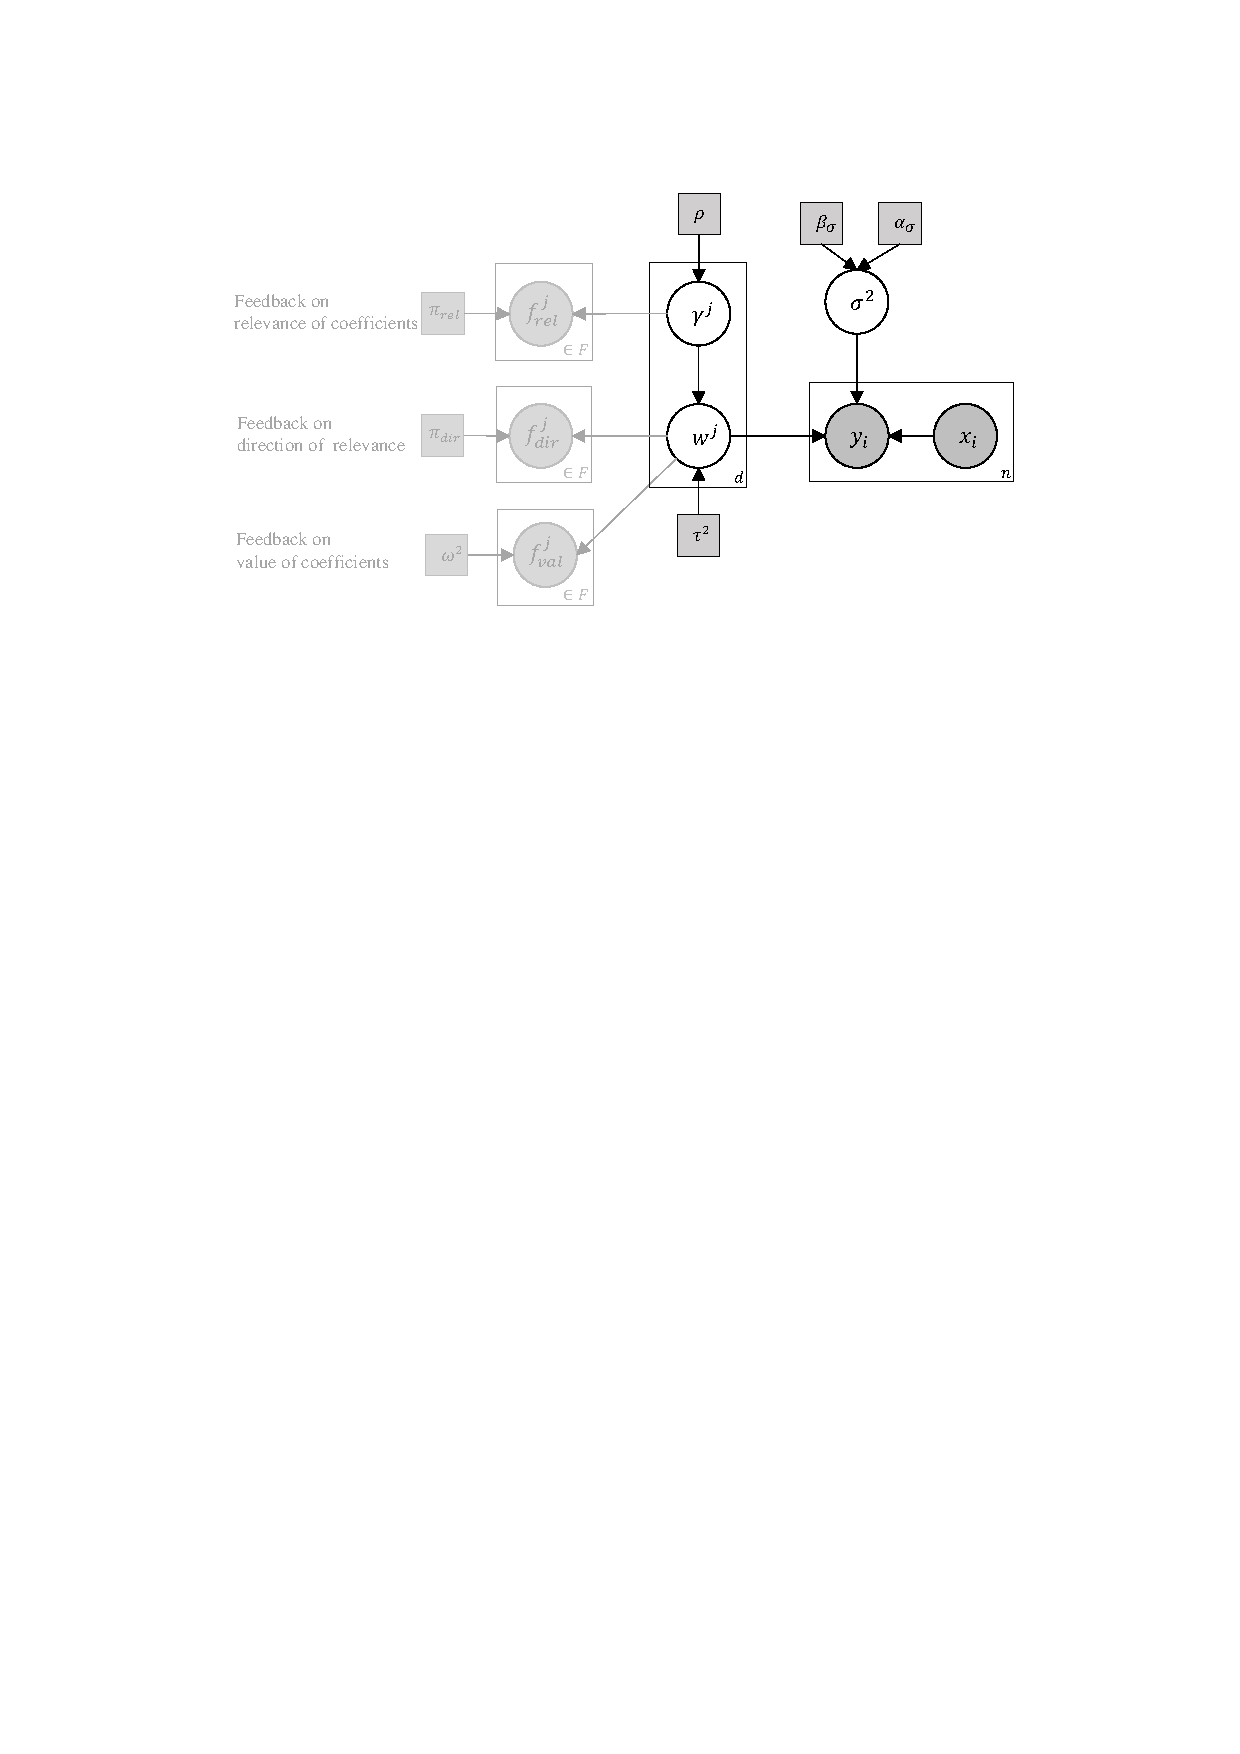
\includegraphics[width=\linewidth]{Figures/Plate_diagram_KE.pdf}
	\caption{Plate notation of the prediction model (Equation \ref{Eq:ss_Bayesian_regression}) and user feedback observations (Equations \ref{Eq:fb_on_val_coeff}, \ref{Eq:fb_on_rel_coeff}, and \ref{Eq:fb_on_dir_coeff}). User provides informative feedback about the model parameters, with the informativeness specified by the dependency assumptions in the figure. %User feedback influences the data model through observations about model parameters.
	Circles represent variables (observed variables are shaded), and shaded squares are the fixed hyperparameters.}
	\label{fig:Plate_KE}
\end{figure}


\begin{itemize}
	\item The user can provide feedback about the value of coefficients
	\begin{equation}\label{Eq:fb_on_val_coeff}
	f_{val}^{j} \sim \normalpdf(w^j, \omega^2),
	\end{equation}
	\noindent where $\omega^2$ models the variance of error in user feedback (noise of the feedback). Knowledge about the value of coefficients is very powerful, however, only available in some specific applications (e.g., exploiting similar trained models or reported coefficient values in related literature).
	 
	\item The user can provide feedback about whether a coefficient should be included or excluded from the model
	\begin{equation}\label{Eq:fb_on_rel_coeff}
	f_{rel}^{j} \sim \gamma^j \bernoullipdf(\pi_{rel}) + (1 - \gamma^j), \bernoullipdf(1 - \pi_{rel}).
	\end{equation}
	\noindent where $\pi_{rel}$ indicates the probability that the user is correct about the feedback. This relevant $f_{rel}^{j}=1$ (or not-relevant $f_{rel}^{j}=0$) feedback is a simple and intuitive form of knowledge that a user may have about a regression task.
	 
	\item The user can provide feedback about the direction of relevance of a coefficient, i.e., whether a feature is positively or negatively correlated with the response variable
	\begin{equation}\label{Eq:fb_on_dir_coeff}
	f_{dir}^{j} \sim I(w^j \geq 0) \bernoullipdf(\pi_{dir}) + I(w^j < 0) \bernoullipdf(1 - \pi_{dir}),
	\end{equation}
	\noindent where $w^j$ is the weight of the $j^{th}$ coefficient and $\pi_{dir}$ indicates the probability that the user is correct about the feedback. Feedback about positive correlation of feature $j$ is coded as $f_{dir}^{j}=1$ and negative correlation as $f_{dir}^{j}=0$.
\end{itemize}



\noindent Connection between the three mentioned feedback models with the data model (Equation \ref{Eq:ss_Bayesian_regression}) is shown as a plate diagram in Figure \ref{fig:Plate_KE}. The full posterior of the unknown parameters given data observations and the user feedback can be described as 

\begin{equation}\label{Eq:Bayes_rule_ss_reg_with_fb}
p(\bw, \bm{\gamma}, \sigma^2 \mid \bD,\bF) = \frac{p(\bD \mid \bw, \sigma^2)p(F_{val} \mid \bw)p(F_{rel} \mid \bm{\gamma})p(F_{dir} \mid \bw)p(\bw \mid \bm{\gamma})p(\sigma^2)p(\bm{\gamma})}{p(\bD,\bF)},
\end{equation} 

\noindent where $F_{val}$, $F_{rel}$, and $F_{dir}$ are the sets of collected feedback corresponding to the three considered feedback types and $\bF = (F_{val}, F_{rel}, F_{dir})$. The  posterior inference is discussed in Section \ref{posteriro_inf}.

%It should be noted that there is no restriction on the amount of feedback (or the types) available for computation of the posterior. 



\subsubsection{Related works}

The proposed feedback models act as communication channels to transfer expert's knowledge to the unknown parameters of the model in an intuitive way. Classical prior elicitation (see for example \cite{OHagan06,garthwaite2005statistical}) aims at eliciting a distribution to represent the expert's knowledge by asking about summary information such as quantiles of the parameters. This is done through iterations between the experts familiar with the data and statisticians who design the model. Our work goes beyond pure elicitation as it directly connects the expert to the probabilistic model, without the need to the statistician. Furthermore, much of the work on elicitation has been designed to maximize accuracy of the prior knowledge, while a focus of our approach is in efficiency of collecting it. By exploiting the training data and available feedback, the probabilistic model can facilitate the interaction with the expert by asking the most important questions first (interaction design will be discussed in Section \ref{interaction}).

We have considered three intuitive types of feedback models. % Studies have shown that the type of domain knowledge in prediction tasks can be summarized in a small set \cite{concept_driven_CHI2019}. 
A different type of feedback is the case where user has knowledge about pairwise similarity of features with respect to the response variable (i.e., asking the user about which  pairs of features affect the prediction output similarly) which has been investigated in \cite{Homayun_pairwise_UMAP,Homayun_pairwise_ijcai2019}. A large body of works have studied the exclusion/inclusion of features (also known as feature selection \cite{Correia2019HumanintheLoopFS}) in different contexts, for classification  \cite{druck2009active,raghavan2006active,settles2011closing}, and regression \cite{Micallef_elicitation}. %These methods are different to ours from the modelling point of view (as we consider sparse models) and also the type of interaction with the user.   
The previous approaches are different to ours from the modelling point of view (as we jointly model the data and user and also investigate a sparse model), the type of feedback, algorithmic solution for real-time performance (will be discussed in Section \ref{posteriro_inf}), and most importantly, the design of interaction between the data model and the user model (will be discussed in Section \ref{interaction}).

\subsection{User feedback as outcome of a cognitive process}

The feedback models proposed in the previous section consider the user as a passive data provider which is not influenced by the interaction. However, humans are active agents which constantly update their knowledge from the interaction. Publication IV investigates a similar knowledge elicitation task to the previous section, but aims at accounting for rational process that humans may undergo during the interaction to produce the feedback. In other words, we will define an active feedback model that accounts for the cognitive process of the user, allowing to gain more information from just a simple feedback.

In many interaction scenarios, such as a visual analytic task or human-in-the-loop machine learning systems, certain aspects of the training data, such as statistics or outputs of the machine learning method, may be revealed to the user  \cite{BEAMES_Endert,sacha2017you,Homayun_pairwise_UMAP,muhlbacher2013partition,Talbot2009,van2011baobabview,Kapoor2010,krause2014infuse,sarkar2015interactive,Micallef_elicitation}. This is mainly done to provide information about important characteristics of the data to improve decision making or to guide the user to facilitate the interaction. For example, in the mentioned knowledge elicitation tasks, the system may first show what it has learned about the coefficients of the linear model from the training data and then ask for user feedback about the same coefficients. This type interaction is prone to overfitting, as the user feedback may not be independent of the knowledge in the training data, while the machine learning methods commonly assume independence between data and user input. Studies in cognitive science have shown that humans are unintentionally biased toward the pieces of information provided for them \cite{Tversky1974,garthwaite2005statistical}. We propose a user model that accounts for such bias. In other words, the user model assumes that the user is rational, in a simple Bayesian sense \cite{gershman2015computational}, and combines the information presented with her knowledge, and then provides the feedback. The user model can then undo the bias in the feedback by performing the inverse of the same rational update.

In particular, we consider the case where the user provides feedback about the probability of relevance of a coefficient. The belief of the model (based on training data alone) about the probability of relevance of the coefficient, i.e., marginal posterior probability $p(\gamma^j \mid \bD)$, is visualized for the user. We make the assumption that the user is rational in combining the visualized information from data with her latent knowledge. The reported feedback is then from the updated knowledge which is partially dependent to the information in the training data. The model should consider this while inferring the posterior of the parameters of interest given the user feedback.
 
\begin{figure}
	\centering
	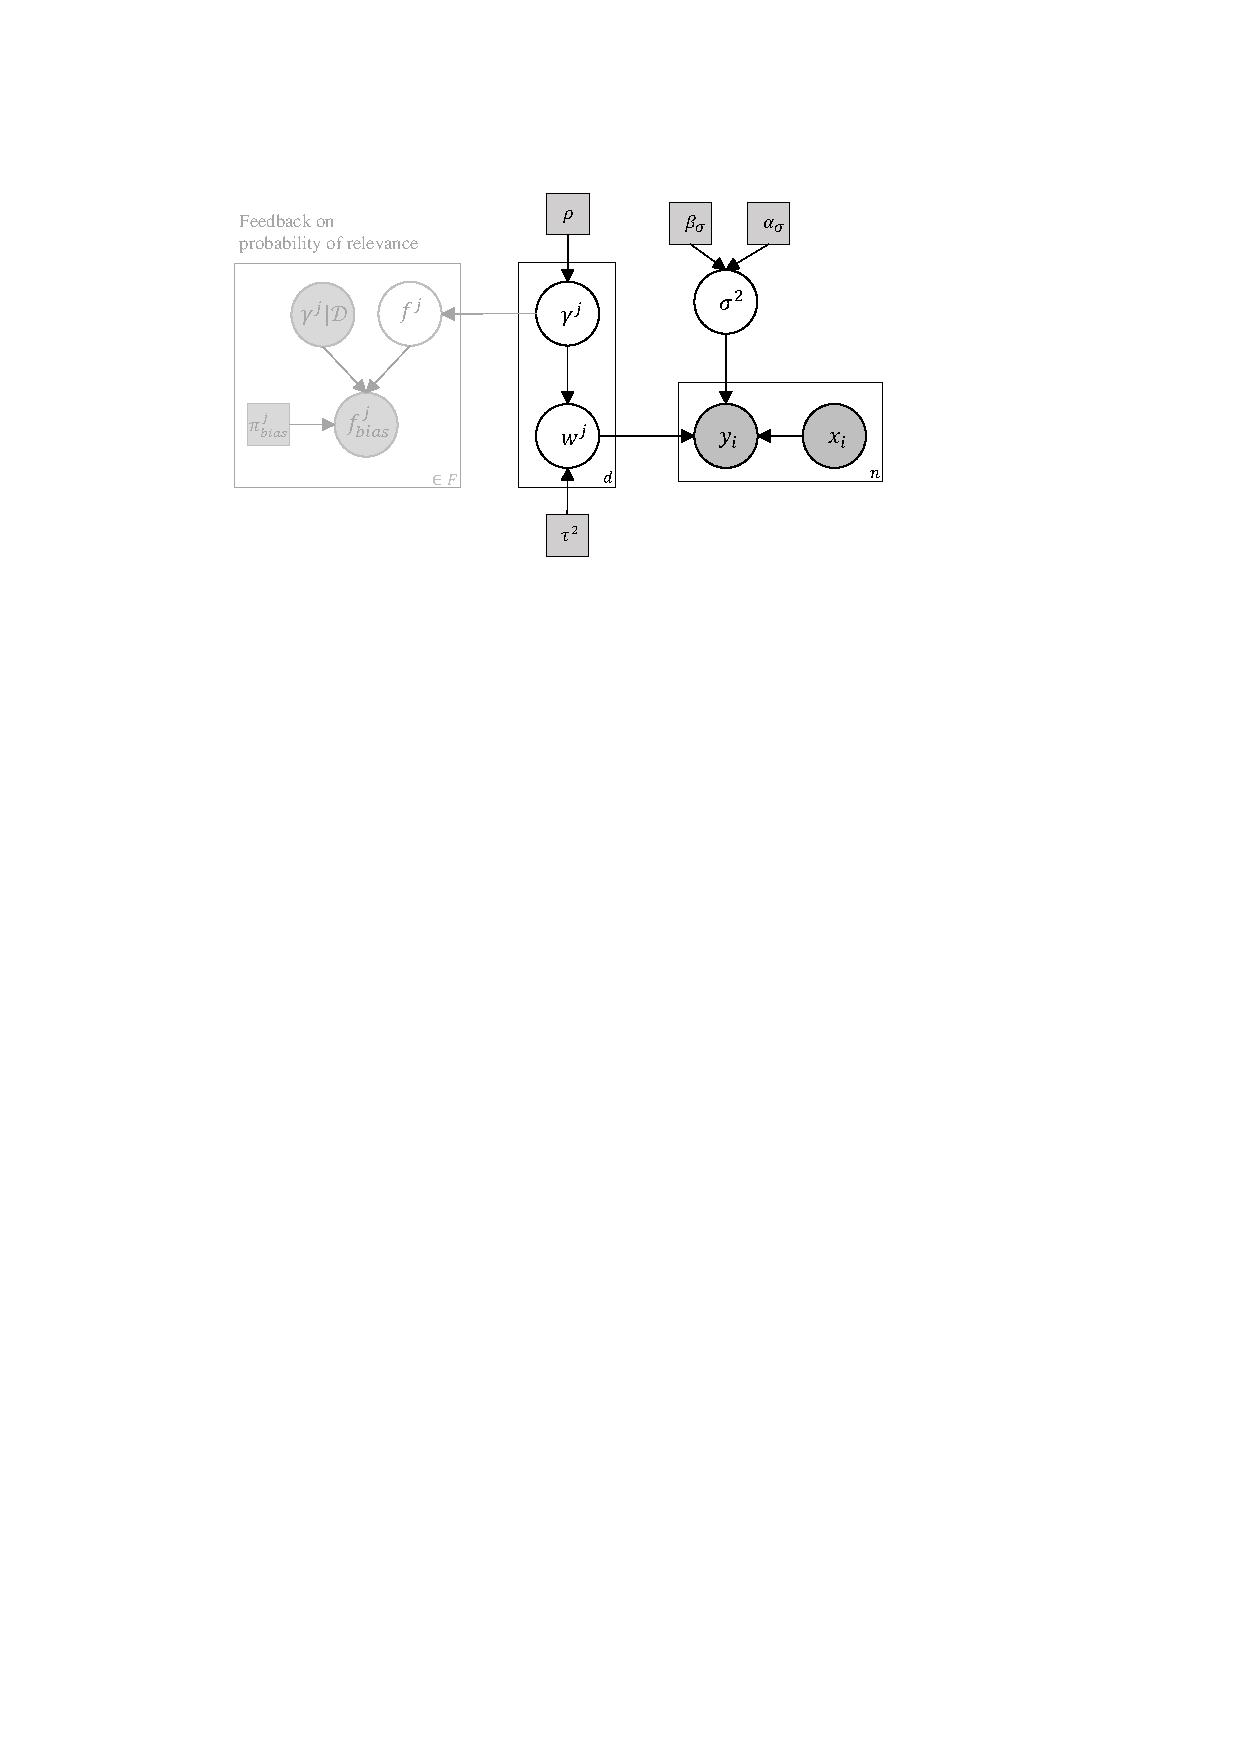
\includegraphics[width=0.80\linewidth]{Figures/Plate_diagram_OF.pdf}
	\caption{Plate notation of the prediction model (see Equation \ref{Eq:ss_Bayesian_regression}) and user model for feedback. The observed user feedback about the probability of relevance of the $j^{th}$ coefficient, $p(\gamma^j \mid \bD,f^j)$, is generated from combination of latent user knowledge about the coefficient, i.e., $p(f^j \mid \gamma^j)$, and information visualized from the data model about probability of relevance of the coefficient, i.e., $p(\gamma^j\mid \bD)$. The user latent knowledge is needed to update the parameters of interest in the data model.}
	\label{fig:Plate_OF}
\end{figure}
 
 
We assume that the user combines her latent knowledge about the probability of relevance of the $j^{th}$ coefficient, i.e., $p(f^{j} \mid \gamma^j=1)$, with the revealed information from the training data, i.e., $p(\gamma^j =1 \mid \bD)$, following a Bayesian update

\begin{equation}\label{Eq:Bayesian_update_biased_fb}
p(\gamma^j=1 \mid \bD, f^{j}) \propto p(f^{j}\mid \gamma^j=1)p(\gamma^j =1\mid \bD),
\end{equation}  

\noindent and provides as feedback the resulting posterior  $p(\gamma^j=1 \mid \bD, f^{j})$. The latent feedback model can be represented as $p(f^{j}\mid \gamma^j) = \pi^j \gamma^j + (1-\pi^j) (1-\gamma^j)$, with $\pi^j$ being the likelihood for latent feedback when $\gamma^j=1$. By doing the inverse of the Bayesian update in \ref{Eq:Bayesian_update_biased_fb}, we can infer $\pi^j$ as:

\begin{equation}\label{Eq:latent_knowledge_infer}
p(f^{j}\mid \gamma^j=1)=\pi^j \propto \dfrac{p(\gamma^j=1 \mid \bD, f^{j})}{p(\gamma^j =1\mid \bD)}.
\end{equation}  

Note that the numerator in \ref{Eq:latent_knowledge_infer} is the observed feedback from the user and the denominator is the model's posterior from the training data, which both are available. We can then use the inferred user feedback $p(f^{j}\mid \gamma^j)$, instead of the observed one, to update the posterior for the parameters of interest. Figure \ref{fig:Plate_OF} depicts a schematic of the data and user model for this problem. Publication IV shows, in a user study, that the prediction performance in a simple sentiment analysis task can be improved if the user model accounts for the rational updates that the user may undergo.

\subsubsection{Related works}

Human biases in interactive tools have been discussed in prior elicitation \cite{garthwaite2005statistical} and visual analytics \cite{bias_warning} fields. In particular, \cite{garthwaite2005statistical} reviews the common human biases from psychological literature and provides guidelines for how to reliably extract expert knowledge about uncertain quantities. In an interactive system implemented in \cite{bias_warning}, the authors proposed a framework for measurement of biases in visual analytics tools and investigated how to inform the user of potential biases. Our work is fundamentally different as we are not limiting (by following a guideline) or interrupting (by showing a warning) the interaction, but rather, acknowledge the presence of such biases and allow the user model, as part of the system, to account for those.

%Several works have investigated methods to extract more from the user feedback alone. Maybe RL works? Our work, is the first to 


\subsection{User feedback for intent modelling}\label{feedback_intent_modelling}

Intent modelling describes the task of learning the hidden intent or interest of a user on a set of items, based on user interaction with those items. Unlike the previous mentioned scenarios where the user interaction used as complementary information to the training data, in Publication I and V the only source of information about the parameter of interest, here intent, is the user feedback on items. An important instance of this scenario is the interactive personalized search systems where in each iteration the system recommends items and the user provides feedback regarding relevance of recommendations. The goal is not just to better predict relevance of items for the user but also to find the most relevant item with minimal interaction. In this section, we discuss the probabilistic modelling of this task and later in Section \ref{MAP_and_BO} discuss how to design the interaction so that the most relevant item can be learned as fast as possible. 

Consider the case where a user is searching for scientific documents by forming a query with keywords. The user might be uncertain about the targeted document or how to express it as keywords, however, for a recommended document, the user can assess its relevance. This information seeking task is usually performed in several iterations starting with an initial query, assessing the recommended results, and modifying the query with the goal of getting better results. This type of information seeking, with the user being uncertain about her information need, is known as exploratory search \cite{Marchionini2006,white2009exploratory} and covers around half of search behaviours of users \cite{Teevan_2004} (see \cite{paba_exploratory_vs_lookup} for in depth review for exploratory and standard lookup search). 

The main bottlenecks of such search systems are that (i) the amount of user feedback gathered on items is very limited compared to the size of the set of all items, and (ii) the users are reluctant to assess more than few recommended items. To tackle these challenges, Publication I exploits the relationship between documents and their keywords and defines feedback likelihoods on both keywords and documents, providing more flexibility for the user to express her intent. Publication V investigates the modelling of noisy implicit, but effortless, feedback generated from brain activity measured through electroencephalography (EEG) and eye movements.  

Formally, the user intent is a relevance profile of all items for the targeted goal. In the document search example mentioned above, the intent can be defined as an unknown function that maps all the keywords %(used to express the search intent) 
and documents to real values, indicating the relevance of each item for the user. Due to receiving limited feedback from the user, it is reasonable to use a simple linear model to represent the intent function. The relation of user feedback on keywords to the intent can be expressed as:

\begin{align}\label{Eq:feedback_on_kw} 
f_{i}^{kw} \sim \normalpdf(\bm{x}_i\tp \bw, \sigma_{kw}^2), 
\end{align}

\noindent where $\bw$ represents the hidden intent and $\sigma_{kw}^2$ models the noise of the keyword feedback. The keywords are represented in the keyword-document matrix $\bm{X} \in \mathbb{R}^{k \times d}$ where the element $(i,j)$ describes weighting of keyword $i$ (out of $k$ total keywords) in document $j$ (out of $d$ total documents), and $\bm{x}_i\tp$ indicates the $i^{th}$ row of the matrix. The values of the keyword-document matrix can be represented by the number of appearances of a keyword in a document or other commonly used statistics such as term frequency–inverse document frequency. 

Intent modelling for document search has previously done at the keyword level \cite{Ruotsalo2018} following \ref{Eq:feedback_on_kw}. However, in this work we are also interested to tie the intent over keywords to documents. We make the simplifying assumption that the expected relevance of a document can be represented as a weighted sum of the expected relevance of keywords that appear in it

\begin{align}\label{Eq:doc_key_relation} 
 \E[f_{j}^{doc}] = \sum_{i=1}^{k} p_{(i \mid j)}  \E[f_{i}^{kw}],
\end{align}

\noindent where $f_{j}^{doc}$ indicates the relevance of the $j^{th}$ document, $\E[.]$ denotes the expected value and $p_{(i \mid j)}$ is the probability of the $i^{th}$ keyword being present in the $j^{th}$ document. The probability $p_{(i \mid j)}$ is not available but can be approximated by normalizing $\bm{X}$ such that its columns sum up to one. Denoting the resulting matrix as $\hat{\bm{X}}$, writing Equation \ref{Eq:doc_key_relation} in vector format, and following  \ref{Eq:feedback_on_kw}, the feedback for relevance of documents can be described as 

\begin{align}\label{Eq:doc_key_relation_vector} 
\bm{F}^{doc} \sim \normalpdf(  \hat{\bm{X}}\tp \bm{X} \bw, \sigma_{doc}^2 \eye),
\end{align}  

\noindent where $\bm{F}^{doc}=[f_{1}^{doc},\ldots,f_{d}^{doc}]\tp$ is the vector representation of relevance feedback for all documents, and $\sigma_{doc}^2$ models the noise of the document feedback. 

\begin{figure}
	\centering
	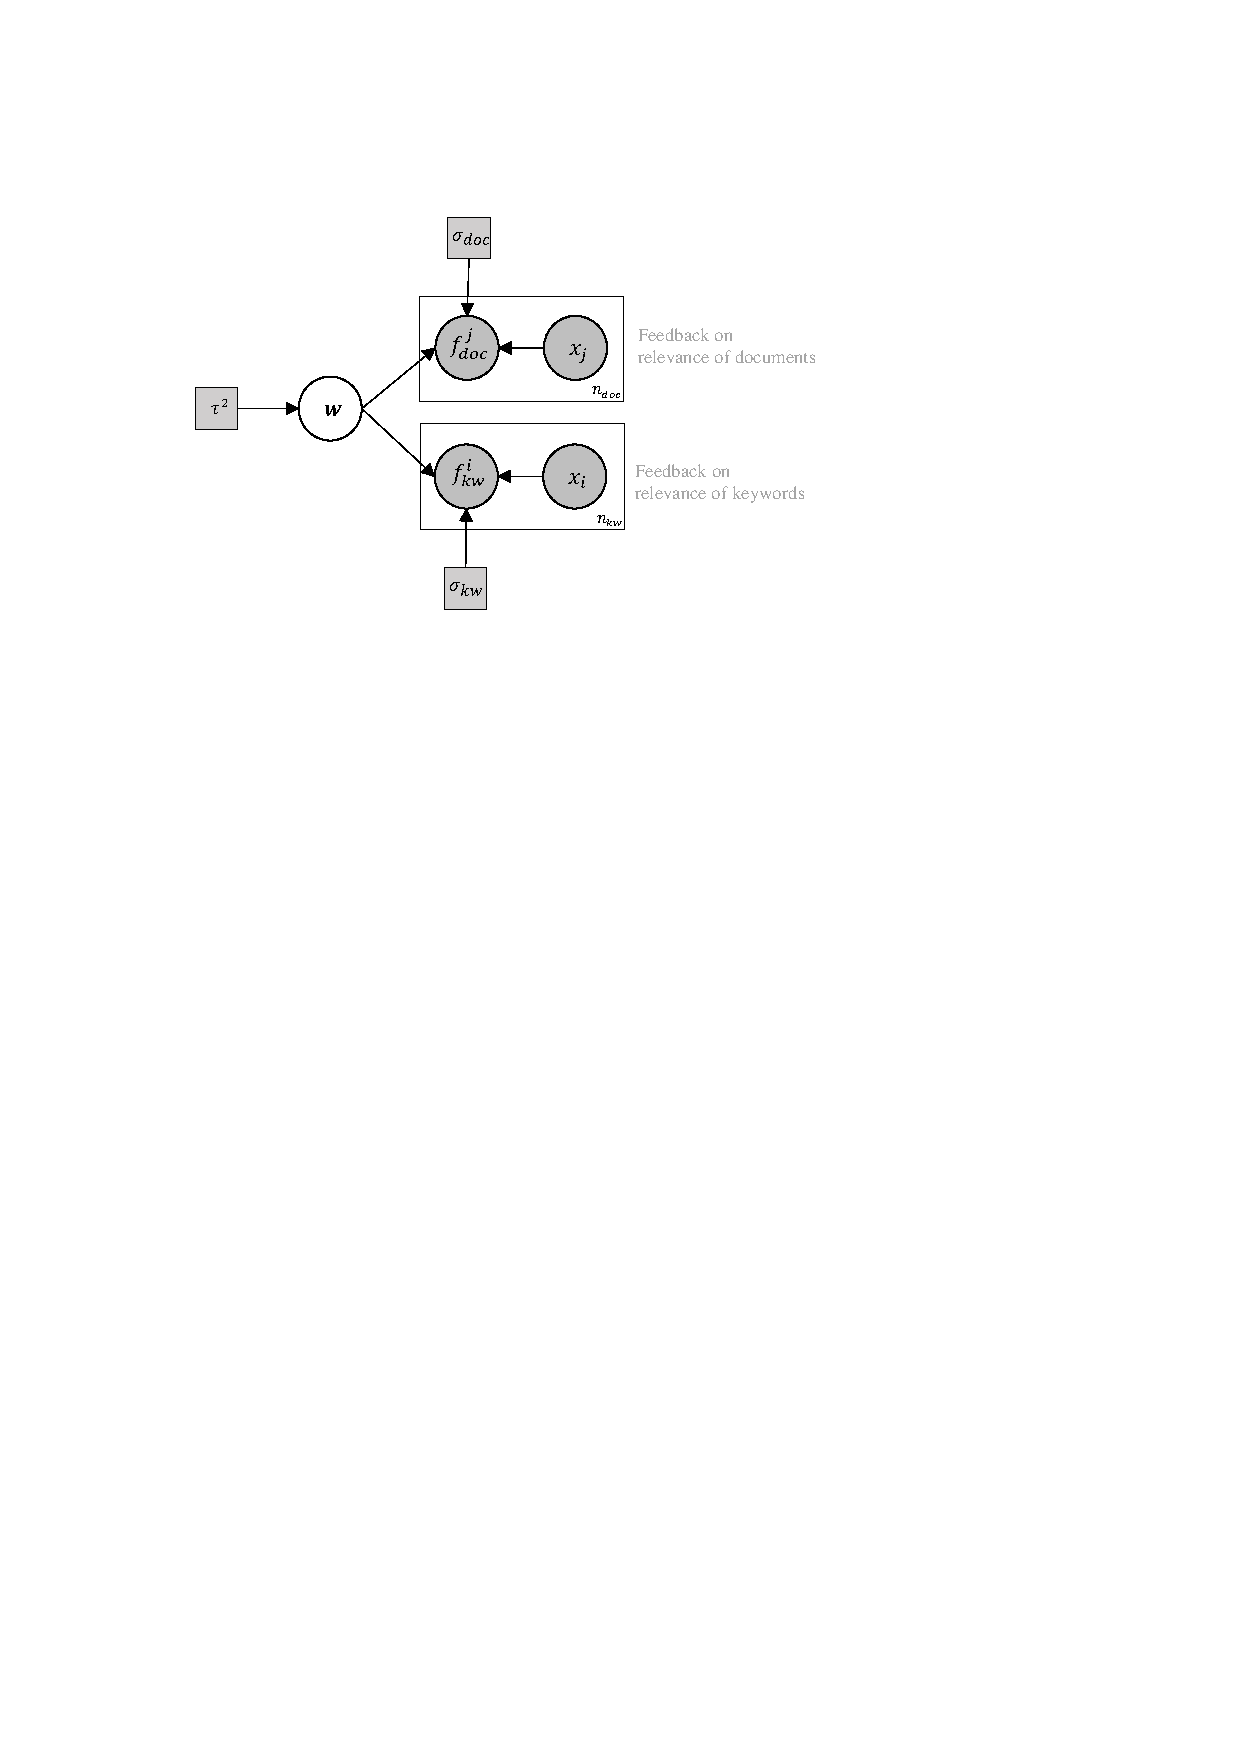
\includegraphics[width=0.80\linewidth]{Figures/Plate_diagram_intent_kd.pdf}
	\caption{Plate notation of the intent modelling from feedback on recommended documents and keywords. The feature transformations are not shown. The feature vector for the $i^{th}$ keyword (shown as $\bm{x}_i$) is the $i^{th}$ column of the keyword-document matrix $\bm{X}\tp$, and for the $j^{th}$ document (shown as $\bm{x}_j$) is the $j^{th}$ column of $\bm{X}\tp\hat{\bm{X}}$.}
	\label{fig:Plate_intent_kd}
\end{figure}

Given user feedback on keywords and documents, the posterior of the hidden intent can be learned by assuming a Gaussian prior on the intent weights, i.e., $\bw \sim \normalpdf(\bm{0},\tau^2 \eye)$. As both likelihoods follow a Gaussian distribution, the posterior has a closed form solution and can be derived following the same derivations as the simple linear model in \ref{Eq:lin_rel_simple_posterior}. Figure \ref{fig:Plate_intent_kd} illustrates the schematic of user feedback models and its connection to the latent intent. 


\subsubsection{Implicit feedback model}

The proposed model is simple as the noise of feedback is assumed to be known and the only unknown parameter is the intent vector $\bw$. As mentioned, we are interested to consider feedbacks from implicit sources such as neurophysiological signals gathered from brain activities. %\footnote{Here we assume that the implicit feedbacks from neurophysiological signals are already converted to a continuous relevance value (see Publication V for details).}. 
These types of implicit feedback require no physical effort from the user, but at the same time are extremely noisy. To exploit this noisy source of feedback along with accurate explicit feedback, we endow the model to decide on the variance of each feedback observation by using the outliers detection model introduced in \ref{Eq:ard_Bayesian_regression}. %to endow the feedback likelihood handle the inherent noise in the implicit feedback when used in combination of the explicit feedbacks.

For simplicity, let's assume that only the keyword feedback is generated from an implicit source (it is straightforward to consider an implicit feedback source for documents or to consider both explicit and implicit feedback for keywords or documents). The implicit feedback likelihood for keywords can be expressed as 

\begin{align}\label{Eq:imp_fb_on_kw} 
f_{i}^{kw} \sim \normalpdf(\bm{x}_i\tp\bw,\frac{\sigma_{kw}^2}{\nu_i}),
\end{align}  

\noindent where the parameters follow the model \ref{Eq:ard_Bayesian_regression}. The model can then infer the accuracy of each feedback, denoted by $\nu_i$, based on the observed feedbacks. The full model for the case of availability of explicit feedback on documents and implicit feedback on keywords is depicted in Figure \ref{fig:Plate_intent_imp}. The resulting posterior is analytically intractable.  

\begin{figure}
	\centering
	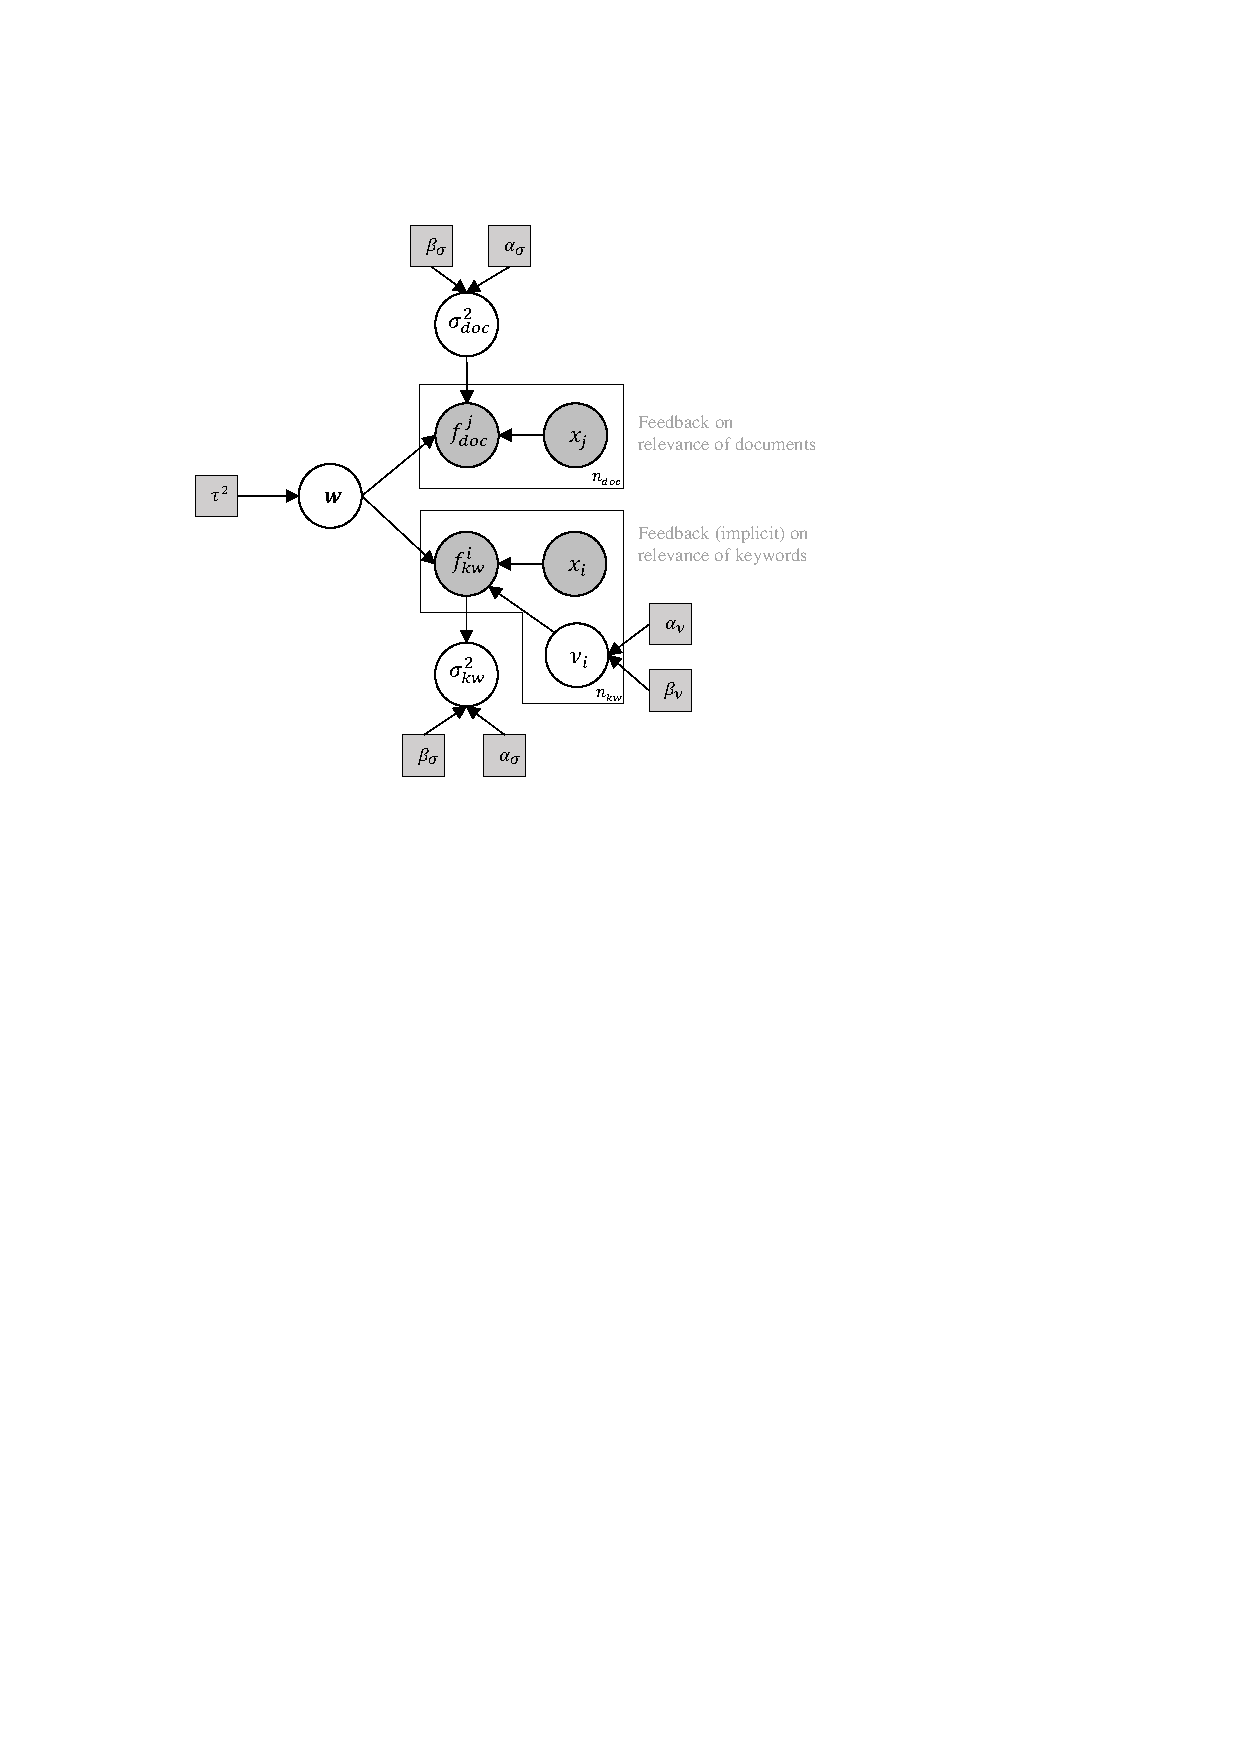
\includegraphics[width=0.80\linewidth]{Figures/Plate_diagram_intent_imp.pdf}
	\caption{Plate notation of the intent modelling from explicit feedback on recommended documents and noisy, implicit feedback on recommended keywords. The model is based on \ref{Eq:ard_Bayesian_regression} with the feedbacks likelihoods following \ref{Eq:imp_fb_on_kw} for keywords and \ref{Eq:doc_key_relation_vector} for documents.}
	\label{fig:Plate_intent_imp}
\end{figure}

   
\subsubsection{Related works}
Intent modelling for personalized document search has been studied in  \cite{GlowIUI2013,ruotsalo2015interactive,Ruotsalo2018}. These works are different to ours as they only define the intent on keywords and use it as an input to a separate retrieval model based on a standard language model, to retrieve ranked documents. We have proposed a natural document likelihood that connects the documents to the intent model which allows the model to directly rank the documents and also to gather user feedback on them. The user interface visualizes the top relevant keywords, suggested by the intent model, on a radar-like interface (borrowed from \cite{GlowIUI2013}) where the distance to the center for each keyword is proportional to the predicted relevance in the intent model. The user can provide explicit feedback by dragging a keyword toward the center (indicating positive relevance) or further away from the center (indicating negative feedback). We considered clicks on a document (to read the document) and bookmarks as positive explicit feedback on the recommended documents which are presented in a list interface. The extraction of implicit relevance feedback from physiological and neurophysiological signals has also been investigated in previous works \cite{OSwald_2015,Manuel2016natural}, but few have attempted to integrate it in a fully integrated information retrieval system as in our work.



\section{Posterior inference} \label{posteriro_inf}
Other than simple models (like the linear regression model introduced in \ref{Eq:lin_rel_simple_posterior}), the models proposed in this thesis do not have a closed-form posterior and posterior predictive distributions. For low-dimensional unknown parameters, it is still practical to approximate the posterior distribution by simulation methods such as numerical computation on grids or Monte Carlo simulations (see \cite[Chapter~10]{Gelman2013} for a review). However, as mentioned, we are interested in high-dimensional problems (e.g., sentiment analysis and search with textual data, or drug response prediction with genomic data), where simple simulation methods cannot scale well due to the curse of dimensionality, i.e., the number of evaluations grows exponentially with respect to the dimension. There are two general families of methods to approach such intractable posteriors, namely Markov chain simulation and deterministic posterior approximation methods.

\subsubsection{Markov chain simulation methods}

Markov chain simulation methods are general methods to draw samples from the target posterior, i.e., $\theta^s \sim p(\theta \mid \bD)$, by starting from an initial sample in the parameter space and sequentially updating the samples toward the target posterior distribution. The updating rule to create the sequence of dependent samples follows the Markov property, i.e., the updating rule to get to $\theta^{t+1}$ at time $t+1$ only depends on the previous sample $\theta^t$, and not the whole chain. %The sequence of dependent samples forms a chain which should have the Markov property, i.e., the updating rule to get to $\theta^{t+1}$ at time $t+1$ should only depend on the previous sample $\theta^t$, and not the whole chain. 
It can be shown, under some assumptions for the updating rule and the Markov chain, that by increasing the chain length toward infinity, the last sample in the chain would be a sample from the target distribution \cite[Chapter~11]{Gelman2013}. Recent advances in Markov chain simulation methods have resulted in probabilistic programming languages, such as Stan \cite{STAN} and Pyro \cite{bingham2018pyro}, that make the computation of Bayesian inference straightforward for end users. The user of such software needs to declare the model as a set of distribution assumptions, and the probabilistic programming language performs the inference by providing samples from the posterior. For example see \cite{Bayesian_workflow_cog_sci_2019} for a step-by-step guides to do Bayesian modelling and inference using Stan. The posterior samples can be used to compute predictive distributions, summaries (such as expected values or other estimates), or utilities for decision making. A bottleneck of iterative simulation methods is that they can sometimes be slow. This is particularly important in the works investigated in this thesis, as all of them require real-time performance with a user.

\subsubsection{Deterministic posterior approximation}

The idea of deterministic approximation methods is to approximate the target distribution, such as posterior distribution $p(\theta \mid \bD)$, with a simpler distribution $q(\theta)$ (e.g., from the exponential family), i.e., $p(\theta \mid \bD) \approx q(\theta)$. The resulting approximation does not fully represent the target distribution; however, in many cases it can be efficient or accurate enough for the targeted task. There are different ways, e.g., different objective functions or assumptions about the approximated distribution, to perform the approximation. Here we briefly review the methods that have been employed in this thesis. 

\paragraph{Variational Bayes (VB)} \cite{Blei_VB} considers $q(\theta)$ from a tractable family and refines it to be similar to the target by minimizing the Kullback–Leibler ($\KLt$) divergence between the approximation and the posterior. $\KLt$-divergence is a popular asymmetric measure of how two distributions are different from each other. For continuous $\theta$ it is defined as\footnote{For discrete $\theta$ the integral turns to summation.} $\KL{q(\theta)}{p(\theta \mid \bD)} \overset{\underset{\mathrm{def}}{}}{=} \int q(\theta) \log\dfrac{q(\theta)}{p(\theta \mid \bD)} d\theta$. This objective is intractable as it requires the computation of the marginal likelihood $\log p(\bD)$. Considering $p(\theta \mid \bD)= \dfrac{p(\theta, \bD)}{p(\bD)}$, the objective can be written as $\KL{q(\theta)}{p(\theta \mid \bD)} = \log p(\bD) - \int q(\theta) \log\dfrac{p(\theta, \bD)}{q(\theta)} d\theta $. Since $\KLt$ is non-negative and $\log p(\bD)$ is constant with respect to $\theta$, the minimization of the $\KLt$-divergence would be equivalent to maximizing $L(q(\theta)) = \int q(\theta) \log\dfrac{p(\theta, \bD)}{q(\theta)} d\theta$. By an appropriate choice for the model family of $q(\theta)$, the maximization of $L(q(\theta))$, also known as evidence lower bound, becomes tractable (unlike the initial objective). In particular, by assuming $q(\theta)$ to factorize into independent parts as $q(\theta) = \prod_{j=1}^{m}q(\theta_j)$, where $\theta_1,\ldots,\theta_m$ are the partitions of $\theta$, 
%$\theta$ can be partitioned into disjoint groups $\theta_1,\ldots,\theta_m$, by assuming factorization $q(\theta) = \prod_{j=1}^{m}q(\theta_j)$, 
a general expression for optimal $q(\theta_j)$, that maximizes $L(q(\theta))$, can be achieved. This approximation is known as the mean-field VB approximation which is implemented by iteratively updating the approximated factors \cite[Chapter~10]{bishop2006pattern}.  
	
Mean-field VB was used in Publication V for the posterior approximation (Equation \ref{Eq:Bayes_rule_ARD}) and for the approximation of the residual variance in the sparse linear model used in Publication II, III, and IV ($\sigma^2$ in Equation \ref{Eq:Bayes_rule_ss_reg_with_fb}).
	
	
\paragraph{Expectation propagation (EP)} \cite{minka2001expectation} aims at finding the $q(\theta)$ that minimizes the $\KLt$-divergence between the posterior and the approximation, i.e., $\KL{p(\theta \mid \bD)}{q(\theta)}$. EP differs from mean-field VB from the objective function point of view, as the inputs of $\KLt$-divergence are reversed, and also in the algorithmic solution of how it is computed. %The minimization is usually intractable. 
EP is suitable for approximating posteriors that can be written in the product form %The posterior distribution can be written as a product of terms 
$p(\theta \mid \bD) = \prod_{j} t_j(\theta)$ (for example the posterior in \ref{Eq:Bayes_rule_ss_reg_with_fb} can be viewed as product of seven terms). It it is sensible to consider the same structure for the approximated posterior $q(\theta) = \prod_{j} \tilde{t}_j(\theta)$. % \dfrac{1}{Z}, where $Z$ is a normalization factor. 
EP approximates each term $t_j(\theta)$ in the posterior by a simpler exponential family form $\tilde{t}_j(\theta)$ such that $\prod_{j} t_j(\theta) \approx \prod_{j}\tilde{t}_j(\theta)$. As the exponential family is closed under products, $q(\theta)$ also follows a simple and tractable exponential form. To optimize the terms, EP iteratively refines the parameters of $\tilde{t}_j(\theta)$ to minimize $\KL{t_j(\theta) q^{\!\!\!\backslash j}(\theta)} {\tilde{t}_j(\theta) q^{\!\!\!\backslash j}(\theta)}$, where $q^{\!\!\!\backslash j}(\theta)$ denotes the approximated posterior after removing the $j^{th}$ term, i.e.,  $q^{\!\!\!\backslash j}(\theta) \propto \frac{q(\theta)}{\tilde{t}_j(\theta)}$. This is optimized by matching the sufficient statistics of $t_j(\theta) q^{\!\!\!\backslash j}(\theta)$ with those of $\tilde{t}_j(\theta) q^{\!\!\!\backslash j}(\theta)$. After refining each $\tilde{t}_j(\theta)$, an updated approximation is achieved as $q(\theta)\propto q^{\!\!\!\backslash j}(\theta) \tilde{t}_j(\theta)$. This step is repeated until convergence of all the terms. \cite{hernandez2013generalized,Lobato2015ML,Tomi_P_thesis}
	
EP can provide a good estimate to uncertainty, e.g., in approximation for the posterior covariance of the weights in the linear model \cite{hernandez2013generalized}. This uncertainty quantification is desirable for designing interaction with a user (experimental design methods; see Section \ref{AL_and_ED}). Furthermore, for sequential interaction, the inference can be sped up by only performing few iterations of parameter updates, instead of waiting for full convergence, as suggested in \cite{seeger2008bayesian}. EP was used in Publications II, III, and IV for fast approximation of the posterior of the sparse linear regression model % with sparsity-inducing spike-and-slab prior on coefficients 
with data and feedback observations (Equation \ref{Eq:Bayes_rule_ss_reg_with_fb}). The regression weights ($\bw$) were approximated by a multivariate Gaussian distribution resulting in Gaussian posterior predictive distributions, which is desirable for fast computation of the experimental design utility (see Section \ref{AL_and_ED}).  
	
%\item Normal (Laplace) approximation where the posterior is approximated with multivariate normal distribution centered at the model of the posterior (see \cite[Chapter~4]{Gelman2013} for a review), 
	
 


%\section{Key components of the joint model}\label{key_comp}








\chapter{User interaction with the probabilistic model}\label{interaction}


 
The previous chapter introduced how the user input to a high-dimensional probabilistic model can jointly be modelled with observational data and how the resulting probabilistic inference can be computed. However, the number of possible feedbacks that a human user can provide is usually limited due to the user's reluctance, e.g., in personalized system the user is usually willing to provide only a couple of feedback, or the time and workload constrains, as there is usually the possibility of providing feedback on thousands of items. To reduce the burden of the user and to reach the target faster, the interaction with the probabilistic model needs to be carefully designed. 

We consider a sequential interaction scenario where at each iteration the probabilistic model selects the next query and the user provides the feedback. The design of the query should be based on the history of observed feedbacks (along with training data, if available) and target of the interaction. Figure \ref{fig:infoflow} depicts a schematic of this interaction. The key components of such an interactive system can be summarized as

\begin{enumerate}
	\item A data observation model $p(\bD \mid \! \theta,\phi_D)$, where the data are in the form $\bD= \{(\bm{x}_i,y_i)\}_{i=1}^{n}$, $\theta$ is the unknown parameter of interest, and $\phi_D$ are model parameters related to data model. The observational data may not be available in some applications (see Section \ref{prob_model_data}). 
	\item A user feedback model $p(f\mid \theta, \phi_F)$, where $\phi_F$ are model parameters related to the user model (see Section \ref{prob_model_user}).
	\item A prior $p(\theta, \phi_D, \phi_F)$ for the hierarchical model description. The data and user model are connected through the shared latent parameter $\theta$.
	\item A query algorithm that facilitates gathering feedback $f$ iteratively from the user (will be discussed in this section).
	\item Bayesian inference for updating the model after user interaction (see Section \ref{posteriro_inf}).
\end{enumerate}

This chapter studies two general families of query algorithms for interaction with the user. A query is a request for information, in the form of feedback, from the user. Section \ref{AL_and_ED} aims at designing a query that maximizes the predictive performance of a probabilistic model. Section \ref{MAP_and_BO} reviews methods for finding the most relevant (rewarding) query with the minimum number of interactions with the user. 


%\vspace{-0.5cm}
\begin{figure}[t]
	\centering
	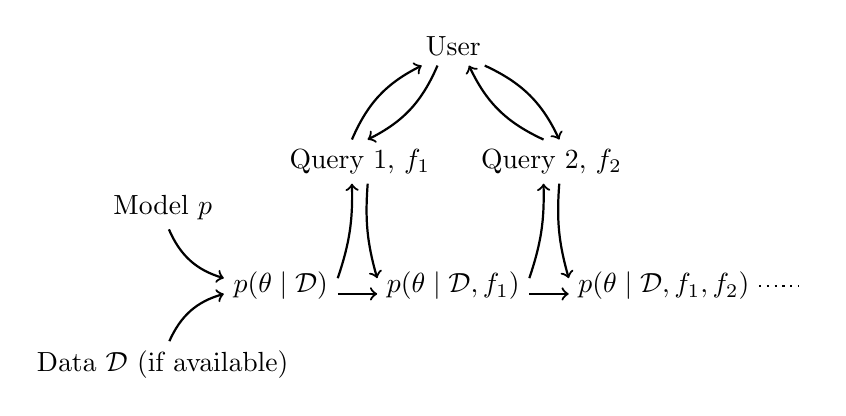
\begin{tikzpicture}[
	%node distance=2.5cm,
	%circle
	]
	\node[] at (-4.5,2) (DM) {Model $p$};
	\node[] at (-4.5,0) (D) {Data $\mathcal{D}$ (if available)};
	\node[] at (-3,1) (p1) {$p(\theta\mid\mathcal{D})$};
	\node[right=0.5cm of p1] (p2) {$p(\theta\mid\mathcal{D},f_1)$};
	\node[right=0.5cm of p2] (p3) {$p(\theta\mid\mathcal{D},f_1,f_2)$};
	\node[right=0.5cm of p3] (p4) {};
	
	\node[above right=1 and 0.28cm of p1,anchor=south] (q1) {Query 1, $f_1$};
	\node[above right=1 and 0.28cm of p2,anchor=south] (q2) {Query 2, $f_2$};
	
	\node[above right=2.5 and 0cm of p2.north,anchor=south,rectangle] (E) {User};
	
	\path[->,bend left=-25,thick] (DM) edge ([yshift=0.1cm]p1.west);
	\path[->,bend left=25,thick] (D) edge ([yshift=-0.1cm]p1.west);
	
	\path[->,thick] ([yshift=-0.1cm]p1.east) edge ([yshift=-0.1cm]p2.west);
	\path[->,thick] ([yshift=-0.1cm]p2.east) edge ([yshift=-0.1cm]p3.west);
	\path[dotted,thick] (p3) edge (p4);
	
	\path[->,bend left=-10,thick] ([yshift=0.1cm]p1.east) edge ([xshift=-0.1cm]q1.south);
	\path[->,bend left=-10,thick] ([xshift=0.1cm]q1.south) edge ([yshift=0.1cm]p2.west);
	
	\path[->,bend left=-10,thick] ([yshift=0.1cm]p2.east) edge ([xshift=-0.1cm]q2.south);
	\path[->,bend left=-10,thick] ([xshift=0.1cm]q2.south) edge ([yshift=0.1cm]p3.west);
	
	\path[<-,bend left=-20,thick] ([xshift=0.1cm]q1.north) edge ([xshift=-0.2cm]E.south);
	\path[<-,bend left=-20,thick] ([xshift=-0.4cm]E.south) edge ([xshift=-0.1cm]q1.north);
	
	\path[<-,bend left=-20,thick] ([xshift=0.1cm]q2.north) edge ([xshift=0.4cm]E.south);
	\path[<-,bend left=-20,thick] ([xshift=0.2cm]E.south) edge ([xshift=-0.1cm]q2.north);
	\end{tikzpicture}
	\caption{Sequential interaction with the user. The probabilistic model uses the history of interaction (and training data, if available) to query the next question from the user and the user provides the corresponding feedback. For brevity, the user and data parameters, $\phi_D$ and $\phi_F$, are omitted from the posterior. See the text for explanation of the notation. The figure is adapted from Publication II.}\label{fig:infoflow}
\end{figure}



\section{Sequential experimental design}\label{AL_and_ED}

In many problems, performing new experiments is expensive. Sequential experimental design \cite{chaloner1995,seeger2008bayesian,settles2010active} (also known as active learning \cite{settles2010active}) is a family of methods that allows the underlying data model to select the next experiment that would maximally improve the model with respect to a utility measure. These methods are usually employed in the data domain, where the model asks the expert to label a new data point (e.g., identifying objects in a picture, flagging an email as spam/no-spam, assessing the sentiment of a text) with the goal to maximally improve the prediction performance of the model. In Section \ref{KE_models}, we considered the interactions at a novel level where the user could provide feedback about model parameters, such as direction of relevance of features. Here we explain how sequential experimental design for such interaction can be designed.


Given the training data $\bD$ and the history of user interactions $\bF$, the aim of our work is to improve prediction on a potential new data such as $(\tilde{\bm{x}},\tilde{y})$. This utility is expressed by the posterior predictive distribution,

%The aim of our work is to improve prediction on data. The prediction on an unobservable data (e.g., test data) given the observed data and also feedbacks form the user is expressed by the posterior predictive distribution of data 

\begin{equation}\label{Eq:post_pred_data_fb}
p(\tilde{y} \mid \tilde{\bm{x}}, \bD,\bF) = \int_{\theta} p(\tilde{y}  \mid \tilde{\bm{x}}, \theta)p(\theta \mid \bD, \bF)d\theta,
\end{equation}

\noindent where $\tilde{y}$ is the unobserved response variable and  $\tilde{\bm{x}}$ is the corresponding feature vector. %, and $\bF$ contains the gathered feedback till now. 
The potential hyperparameters for user and data models ($\phi_f$ and $\phi_D$) are omitted for brevity. 

The goal of interaction is to query the user such that the corresponding user response would maximally improve the above predictive distribution. The queries are asked about the feature as explained in Section \ref{KE_models}. %The goal is to query the user about the feature, let's say $j^*$, that the corresponding feedback, i.e., $f^{j^*}$, would maximally improve the above predictive distribution.
The improvement can be measured by comparing the posterior predictive distribution after and before receiving the feedback, using $\KLt$-divergence, i.e., $\KL{p(\tilde{y} \mid \tilde{\bm{x}}, \bD,\bF,f^{j})} {p(\tilde{y} \mid, \tilde{\bm{x}}, \bD,\bF)}$, where $f^{j}$ is the user feedback after querying feature $j$. This utility is known as the information gain and it measures the impact of the new feedback on the posterior predictive distribution of the data. Information gain cannot be computed as (i) the unobserved data $(\tilde{\bm{x}},\tilde{y})$ is not usually available, and (ii) the user feedback $f^{j}$ is observed only after querying $j$ from the user. Rather than computing the utility on unobserved data, we use the available training data set. Furthermore, unobserved feedback can be handled by computing the expected feedback that the user may provide after the query. This expectation would be taken with respect to the posterior predictive distribution of user feedback which is the distribution that the system believes the feedback would be generated from, i.e., the user model $p(\tilde{f}^j \mid \bD,\bF)= \int_{\theta} p(\tilde{f}^j \mid \theta)p(\theta \mid \bD, \bF)d\theta$. The best query can then be  selected as

\begin{equation}\label{Eq:expected_info_gain}
j^* = \argmax_{j \notin \bF} \E_{p(\tilde{f}^j \mid \bD,\bF)} \left[ \sum_{i=1}^{n}  \KL{p(\tilde{y}\mid \bm{x}_i, \bD,\bF,\tilde{f}^j)} {p(\tilde{y} \mid \bm{x}_i, \bD,\bF)} \right].
\end{equation}
    
This new utility, known as expected information gain, is expensive to compute. For each potential query, it requires the computation of the posterior predictive distribution before and after the new feedback (which itself requires the computation of the corresponding posterior and solving the integral in Equation \ref{Eq:post_pred_data_fb}), computation of the $\KLt$-divergence, and computation of the posterior predictive distribution of the feedback necessary for deriving the expectation. 


Publications II and III used expected information gain to sequentially extract the experts' knowledge about the model (see Section \ref{KE_models} for a summary about the types of knowledge extracted). The real-time computation was realized by approximating the posterior by a multivariate Gaussian distribution using the EP algorithm which resulted in simple forms for posterior predictive distributions and an analytical solution to the $\KLt$-divergence.   

%Publications II and III used expected information gain to sequentially extract the experts' knowledge about model (see Section \ref{KE_models} for a summary about the types of knowledge extracted). The posterior distribution of the weights of the linear model \ref{Eq:Bayes_rule_ss_reg_with_fb} is approximated by a multivariate Gaussian distribution using the EP algorithm. 
%Given this approximation, it is straightforward to show that the posterior predictive distribution of the data also follows a Gaussian distribution which gives an analytical solution to the $\KLt$-divergence. The posterior predictive distribution of feedback observations follows a Gaussian distribution (for feedback on value of coefficients) or a Bernoulli distribution (for feedback on relevance and direction of relevance of coefficients). Consequently, the computation of the expected information gain \ref{Eq:expected_info_gain} becomes straightforward and can be performed in real-time.
 

\section{Multi-armed bandits and Bayesian optimization}\label{MAP_and_BO}

Consider the optimization problem $x^* = \argmax_{x \in \mathcal{X}} f(x)$, where $\mathcal{X}$ is the design space, and $f(.)$ is the function of interest. In many applications the target function is unknown and expensive to evaluate. For example, $f(.)$ can represent user interest over a set of items where the only way to evaluate it is to query the user with an item $x_q \in \mathcal{X}$ and observe the corresponding feedback $f(x_q)$. The goal of such black box optimization problem could be to find the highest point of the function $x^*$ with as few function queries as possible. This problem has been extensively investigated in the multi-armed bandit \cite{bubeck2012regret} and Bayesian optimization \cite{brochu2010tutorial,BO_review} literatures. Due to limited query budget, these methods need to compromise between querying points that provides new information about the target function in less-explored areas, versus exploiting the current best estimates about the position of the maximum. 
%Consider the problem of finding the argument that maximizes an objective function in a design space $\mathcal{X}$, i.e., $x^* = \argmax_{x \in \mathcal{X}} f(x)$. Now consider that the function of interest $f(x)$ is unknown and expensive to evaluate, and the only way to gain information about it is to sequentially query it, i.e., ask the function value about a point of interest, such as $x_q \in \mathcal{X}$, and observe the corresponding function value $f(x_q)$ (or in general a noisy version of it). The natural goal for this black box optimization problem could be to find $x^*$ with the minimum number of queries. This problem has been extensively investigated in the multi-armed bandit \cite{bubeck2012regret} and Bayesian optimization \cite{brochu2010tutorial,BO_review} literatures. A core characteristic of these approaches is that they need to make a compromise between asking queries that would provide new information about the hidden objective function (for example in areas that have not been explored), versus exploiting the current best guess about the position of the maximum. 
This is known as the exploration exploitation trade-off and methods in the literature propose different query strategies, known as acquisition functions, to balance it. Bayesian optimization and multi-armed bandits methods have been used in many applications such as clinical trials for finding the best treatment for a patient out of several alternatives \cite{bubeck2012regret}, ad placement for finding the ad that would have the highest user click chance \cite{Bandit_IR}, Automatic machine learning for searching in space of machine learning models \cite{hoffman2014correlation}, reinforcement learning for finding the best action of an agent \cite{brochu2010tutorial}, design of new materials \cite{frazier2016bayesian,BOSS2019}, and personalized search systems \cite{ruotsalo2015interactive}. 

A focus of this thesis is personalized search systems, where the goal is to find the most relevant item for a user with minimum interaction. One can map this problem to the black-box optimization problem introduced above as the user relevance profile over items is unobserved and can only be queried, i.e., querying an item $\bm{x}$ and observing the corresponding feedback $f$. In particular, the problem can be formulated as finding (recommending) the item that has the highest expected relevance or equivalently highest expected feedback value. We mainly study linear models %As explained in Section \ref{feedback_intent_modelling}, we consider the cases
where the expected relevance of items have a linear relationship with the unknown parameter $\bm{\theta}$\footnote{Note that we have changed the notation for the unknown weight vectors $\bm{w}$ in Section \ref{prob_model_user} to $\bm{\theta}$ for consistency.} that expresses the user intent. The optimization can then be described as finding the $\bm{x}^*$ for which: 

\begin{equation}\label{Eq:black_box_optimization}
\bm{x}^* = \argmax_{\bm{x} \in \mathcal{X}} \E [f \mid \bm{x}] = \argmax_{\bm{x} \in \mathcal{X}} \bm{x}\tp \bm{\theta}.
\end{equation}

Given a history of interaction at time $t$, $\bF_t = \{(\bm{x}_i , f_i)\}_{i=1}^{t}$, the loss of the query algorithm can be measured by the expected cumulative regret defined as:

\begin{equation}\label{Eq:regret}
\textrm{regret}_t = t \bm{x}^{*\top} \bm{\theta} - \sum_{i=1}^{t} \bm{x}_i\tp \bm{\theta}.
\end{equation} 

\noindent Note that the cumulative regret is minimized if the most relevant item is recommended to the user. The relevance profile of the user over items is determined by $\bm{\theta}$. Since we are using Bayesian statistics, we have an ongoing posterior given the history of user feedback $p(\bm{\theta} \mid \bF_t)$ which can help us to better design the next query to ask from the user. % due to having an immediate expression of the uncertainty about $\bm{\theta}$. 
There are different forms of acquisition functions that exploit the model uncertainty to design the next query. Two common ones are upper confidence bound (UCB) \cite{auer2002using,Bayes_UCB} and Thompson sampling \cite{agrawal2013thompson}, which both enjoy theoretical guarantees (for some family of problems) regarding how well they control the regret. 

Publications I and V used Thompson sampling to balance the exploration and exploitation of the recommendations. Thompson sampling follows the probabilistic idea and selects the next query according to its posterior probability of being the best query:  

\begin{equation}\label{Eq:Thompson}
\Pr(\bm{x}_{q})=\!\!\int_{\bm{\theta}}\!\!I(\argmax_{\bm{x} \in \mathcal{X}} \bm{x}\tp \bm{\theta} \!=\!\bm{x}_{q}\!\!\mid \!\bm{\theta}) p(\bm{\theta} \mid \bF_t) d\bm{\theta},
\end{equation}
 

\noindent where $\Pr(\bm{x}_{q})$ is the Thompson probability for selecting query point $\bm{x}_{q}$, and $I(.)$ is the indicator function which returns 1 if the condition in front of it holds and zero otherwise. Selection of the query at time $t+1$ according to the Thompson probabilities can be realized through the following steps:

\begin{enumerate}
	\item Draw a sample from the posterior: $ \bm{\theta}^s \sim p(\bm{\theta} \mid \bF_t)$.
	\item Find the query that has the highest expected relevance given the posterior sample: $\bm{x}_{q} = \argmax_{\bm{x} \in \mathcal{X}} \bm{x}\tp \bm{\theta}^s$.
	\item Ask the query from the user, observe the user feedback, and update the posterior given the new observation: $p(\bm{\theta} \mid \bF_{t+1})$, where $ \bF_{t+1} = \bF_{t} \cup \{(\bm{x}_{q},f_q)\}$.
\end{enumerate}

In Publications I and V we considered expected feedback models for items, i.e., keywords and documents, which had a linear relation with the unknown intent parameter (see likelihoods  \ref{Eq:feedback_on_kw}, \ref{Eq:doc_key_relation_vector}, and \ref{Eq:imp_fb_on_kw} in Section \ref{feedback_intent_modelling}.). Thus, the same algorithm can be applied with the addition that at each iteration different query types (documents and keywords) are selected to be recommended to the user.


\chapter{Summary of the contributions}
%Summary of the Contributions
%Applications and results OR Summary of the Publications
%Go through the papers and tasks. 
This chapter briefly summarizes the contributions of Publications I-V with emphasis on answering the research questions of the thesis. %The thesis is concluded with a discussion.

\section{Interactive intent modelling from multiple feedback domains (Publications I and V)}


RQ1 was ``Can we facilitate interactive intent modelling by adding new interaction domains?''

Publications I and V investigated the ways to improve interactive intent modelling by considering new feedback domains. The application considered in these papers was a personalized document search problem where at each iteration the system recommends a list of documents and keywords, given the history of user interaction, and the user provides feedback to them with the goal to find the most relevant document faster.

In particular, Publication I exploited the relationship between documents and keywords and proposed a joint probabilistic model that ties the user feedback on both keywords and documents (see Figure \ref{fig:Plate_intent_kd} for model description) to the latent user intent. Previous works \cite{GlowIUI2013,ruotsalo2015interactive} only defined the user intent on keywords and had a separate language model to retrieve documents. The joint probabilistic model allows to learn the user intent with fewer interaction rounds and at the same time provides a unified way to recommend keywords and documents by using Thompson sampling on the posterior of the latent intent (see Section \ref{MAP_and_BO} for details). The model was evaluated in a simulated study and a user study with 10 participants using the exploratory search system SciNet \cite{GlowIUI2013}. 

Publication V investigated the inclusion of noisy neurophysiological signals gathered from brain activities as a new source of feedback, along with scarce explicit interactions. Both feedback types were gathered on the same domain of items, however, the different nature of noise made the integration challenging.  
%The feedback was in the same domain of items but, compared to the previous work, its generating nature was assumed to be implicit. The integration of feedbacks is challenging due to different nature of noise. 
To enable the model to account for the noisy feedback, we considered a per-observation noise parameter that controls the variance of feedback. 
%To account for the noisy feedback we considered a per feedback prior parameter that controls the noise of the feedback, given the feedback source. 
The posterior of that parameter determines the accuracy of the feedback and allows the model to discard outlier feedbacks which are common in neurophysiological sources (see Figure \ref{fig:Plate_intent_imp} for model description). We used the same approach as Publication I to connect the feedback on documents and keywords and to recommend new items. The model was evaluated in a user study with 16 participants in a first-of-its-kind fully integrated information retrieval system that used the real-time generated feedback from brain activities (EEG) and eye movements tracking (to map the brain signal to visualized items), and scarce mouse click feedback.

The conclusion to RQ1 is that, interactive intent modelling can benefit from adding new domains of feedback as long as the uncertainty of the feedback source and connection of the feedback to the latent intent is properly accounted for. In particular, we modeled both the user interaction and recommendation in one probabilistic model. This is particularly important as recommendation based on exploration-exploitation principle is fundamentally guided through the uncertainty. Having a joint probabilistic model of both the user and the task allows the uncertainty to accurately propagate in the recommendation and results in more efficient exploration. 


\section{Expert knowledge elicitation for high-dimensional prediction (Publications II and III)}

RQ2 was ``Can we improve prediction performance by directly extracting expert knowledge about the model?''

Publications II and III studied the ways user knowledge about the parameters of a model can be encapsulated as likelihood functions and how they can sequentially be queried to improve the performance of a prediction task. Expert knowledge is particularly important in ``small $n$, large $p$'' scenarios where the number of available data points ($n$) is fewer than the dimension of the problem ($p$). An example application that was investigated in Publication III is the drug response prediction given few patient profiles, where it is very costly, or in some cases impossible, to add new data to the training data set but expert knowledge is available. 

Both publications contributed to the research question by introducing feedback models for extracting expert knowledge (see Figure \ref{fig:Plate_KE} for the three suggested feedback types) and designing the interaction with sequential experimental design to query the most informative expert knowledge earlier (see Section \ref{AL_and_ED} for details). Both publications were evaluated by extensive simulated experiments and studies with real users/experts.

In conclusion, the experiments in these works indicate that (i) adding expert feedback, in a joint probabilistic model of user and data, improves the prediction performance of the model. In particular, publication II compares the amount of improvement from adding new feedback to the improvement achieved by adding new data observation in two sentiment analysis tasks. The results show that even though the improvement from adding new data points is usually higher than adding new feedbacks, the amplitude of improvements are still comparable. This is very valuable as in many applications adding intuitive expert feedback is cheaper than adding new data points. (ii) The order of queries from the experts significantly affects the improvement rate. In particular, compared to a random query the improvement rate is more than four times higher during the initial queries using the proposed sequential experimental design.

%The conclusion to RQ2 is that, even though the expert knowledge is not as powerful as new labeled data points, if connected properly to the data model, the knowledge can still significantly improve the prediction performance on high-dimensional small datasets. This increase in performance is noticeably fast if the queries are designed sequentially by the model so that the most informative questions are queried first. 



\section{User modelling beyond passive feedback provider in knowledge elicitation (Publication IV)}

RQ3 was ``Is it beneficial to model the expert as an active agent that updates its knowledge during knowledge elicitation?''

Publication IV investigates the complementary question to RQ2 of what if we acknowledge that the knowledge elicitation is being performed on a human user which comes with their own preset of biases and cognitive characteristics. We considered anchoring bias as one of the well-studied cognitive biases \cite{Tversky1974} and ask what if the knowledge elicitation system explicitly accounts for this behaviour while gathering user feedback. In particular, while querying the user about the model, some aspects of the training data, such as statistics or scatter plots, may be revealed to the user. 
%The bias can particularly be harmful when extracting user knowledge after revealing certain aspects of training data, such as statistics or scatter plots. If not accounted properly, 
the user knowledge can be influenced by the information in the training data which makes the extracted knowledge dependent to the training data. This dependency is undesirable as most human-in-the loop systems model the user inputs as an independent source of information. Rather than alarming the user about this potential defect \cite{bias_warning}, we proposed a probabilistic model that acknowledges the dependency. The user model assumes that the user updates her latent knowledge with the information in the training data that has been revealed and provides the feedback based on the updated knowledge. The model then accounts for the dependency by performing the inverse of the knowledge update. This allows the user model to extract the tacit knowledge (see Figure \ref{fig:Plate_OF} for model description). The proposed user model was evaluated on a simple user study with 49 participants and the results showed that modelling the user's thinking behaviour in knowledge elicitation improves the prediction performance.

The conclusion to RQ3 is that interactive models can gain more from an observed user feedback if they correctly model the unobserved thinking process that the user may undergo to produce the feedback. The finding is striking as it opens a new horizon for user modelling in human-in-the-loop machine learning systems where the user model acknowledges how the human interacts and is able to condition on the thinking process to have more informative updates from an observed interaction.

\chapter{Discussion}

The thesis has focused on modelling the user interaction with a machine learning system as a unified probabilistic model of both the user model, i.e., model of user interaction in the form of feedback and intention, and the data model. The user interaction with the model has then been designed as a sequential probabilistic inference problem where the most informative query from the user is selected at each iteration (see Figure \ref{fig:infoflow}). The thesis contributes to the fields of human-in-the-loop machine learning and human-computer-interaction from several aspects.

Few works have investigated the benefits of explicitly modelling human aspects in the human-in-the-loop machine learning methods. In \cite{NIPS2016_6155} the authors noted that humans are sometimes uncertain about the label of some queries in an active learning scenario and only later accumulate enough information to be able make such label decisions. They investigated the query complexity of active learning under such human behaviour. In a later work \cite{peltola2019machine}, we showed that the performance of a personalized search system can be improved if the user model acknowledges that the user is also modelling the system they are interacting with and exploiting this knowledge in their interaction. 

We believe that probabilistic user modelling would be of great importance in human-in-the-loop machine learning systems as it allows to (i) infer more information from an observed user feedback and (ii) design better interactions by exploiting the quantified uncertainty. User modelling, can provide the machine with a model of how users perceive the world, and the works in this thesis show that exploiting this knowledge can improve the interaction.
%\paragraph{Human-computer-interaction} 
%TODO: add moer discussion. see other people's thesis




%--------------------------------END--------------------------%


 % Refer to the Journal paper 1 of this example document
%\citepub{j1} \& \cpub{j1} \& \cp{j1} \& \pageref{j1} \& \ref{j1}
% Refer to the Conference paper of this example document
%\citepub[p.~2]{c1} \& \cpub[Sec.~ 1]{c1} \&  \cp[pp.~1--2]{c1} \& \pageref{c1} \& \ref{c1} 


\renewcommand{\bibname}{References}
\bibliographystyle{plain} % Change as required
\LARGE\bibliography{references}  % remember to edit the file name




%% The following commands are for article dissertations, remove them if you write a monograph dissertation.

% Errata list, if you have errors in the publications.
%\errata

%% The first publication (journal article)
% Set the publication information.
% This command musts to be the first!
\addpublication[conference]{\underline{Pedram Daee}, Joel Pyykk\"o, Dorota G\l{}owacka, and Samuel Kaski}{Interactive Intent Modeling from Multiple Feedback Domains}{Proceedings of the 21st International Conference on Intelligent User Interfaces}{Sonoma, California, USA, pages 71--75}{March}{2016}{ACM.}{c1}

%\addpublication{Journal Paper Authors}{Journal Paper Title}{Journal Name}{Volume, issue, pages, and other detailed information}{Month}{Year}{Copyright Holder}{j1}
%\addpublication[conference]{Conference Paper Authors}{Conference Paper Title}{Conference Name}{Location, pages, and other detailed information}{Month}{Year}{Copyright Holder}{c1}
%\addpublication[accepted]{Journal Paper 2 Authors}{Journal Paper 2 Title}{Journal Name 2}{}{Month}{Year}{Copyright Holder}{j2}
%\addpublication[submitted]{Journal Paper 3 Authors}{Journal Paper 3 Title}{Journal Name 3}{}{Submission date}{Year}{No copyright holder at this moment}{j3}
% Add the dissertation author's contribution to that publication (the order can be interchanged with \adderrata).
\addcontribution{The author had the main responsiblity in problem formulation and modelling. The author designed and implemented the simulation experiment. Joel Pyykk\"o and the author built the system for user studies and conducted the studies together. The author wrote the initial draft of the manuscript, after which all co-authors joined for revisions.}
% Add the errata of the publication, remove if there are none (the order can be interchanged with \addauthorscontribution).
%\adderrata{j1 I This is wrong}
% Add the publication pdf file, the filename is the parameter (must be the last).
%TODO: uncomment the following in the final version (now commented to increase speed)
\addpublicationpdf{Articles/IUI16.pdf}



\addpublication[journal]{\underline{Pedram Daee}, Tomi Peltola, Marta Soare, and Samuel Kaski}{Knowledge elicitation via sequential probabilistic inference for high-dimensional prediction}{Machine Learning}{volume 106, issue 9-10, pages 1599--1620}{}{2017}{Copyright belongs to the authors.}{j1}
\addcontribution{The ideas and experiments in this article were designed jointly (the first three authors contributed equally). The author had the main responsibility in the derivation of the sequential experimental design and implementation of the experiments. Dr. Tomi Peltola derived and implemented the posterior approximation. The manuscript was written jointly.}
%TODO: uncomment the following in the final version (now commented to increase speed)
\addpublicationpdf{Articles/ML17.pdf}



\addpublication[journal]{Iiris Sundin, Tomi Peltola, Luana Micallef, Homayun Afrabandpey, Marta Soare, Muntasir Mamun Majumder, \underline{Pedram Daee}, Chen He, Baris Serim, Aki Havulinna, Caroline Heckman, Giulio Jacucci, Pekka Marttinen, and Samuel Kaski}{Improving genomics-based predictions for precision medicine through active elicitation of expert knowledge}{Bioinformatics}{volume 34, issue 13, pages i395–i403}{}{2018}{Copyright belongs to the authors.}{j2}
\addcontribution{The author contributed on formulating the sequential experimental design and implementing a portion of the early version of the experiments. The author commented on the manuscript.}
%TODO: uncomment the following in the final version (now commented to increase speed)
\addpublicationpdf{Articles/Bio18.pdf}


\addpublication[conference]{\underline{Pedram Daee}, Tomi Peltola, Aki Vehtari, and Samuel Kaski}{User Modelling for Avoiding Overfitting in Interactive Knowledge Elicitation for Prediction}{Proceedings of the 23rd International Conference on Intelligent User Interfaces}{Tokyo, Japan, pages 305--310}{March}{2018}{ACM.}{c2}
\addcontribution{The problem formulation was a joint effort (the first two authors contributed equally). The author designed, implemented, and carried out the user experiment. Dr. Tomi Peltola derived and implemented the posterior approximation. The first two authors wrote the initial draft of the manuscript, after which all co-authors joined for revisions.}
%TODO: uncomment the following in the final version (now commented to increase speed)
\addpublicationpdf{Articles/IUI18.pdf}


\addpublication[journal]{Giulio Jacucci, Oswald Barral, \underline{Pedram Daee}, Markus Wenzel, Baris Serim, Tuukka Ruotsalo, Patrik Pluchino, Jonathan Freeman, Luciano Gamberini, Samuel Kaski, Benjamin Blankertz}{Integrating Neurophysiological Relevance Feedback in Intent Modeling for Information Retrieval}{Journal of the Association for Information Science and Technology}{volume 70, issue 9, pages 917--930}{}{2019}{Copyright belongs to the authors.}{j3}
\addcontribution{The author had the main responsibility in designing and implementing  the interactive intent modelling and information retrieval system, and writing of the corresponding sections. All authors contributed to paper revisions.}
%TODO: uncomment the following in the final version (now commented to increase speed)
\addpublicationpdf{Articles/JASIST19.pdf}

%% The fourth publication (yet another journal paper, submitted for publication, note the optional parameter)
%% Note that you are allowed to use this option only when submitting the dissertation for pre-examination!
% Set the publication information, detailed information is not printed
%\addpublication[submitted]{Salvatore Andolina$^*$, \underline{Pedram Daee}$^*$, Tung Vuong$^*$, Tuukka Ruotsalo, Khalil Klouche, Mats Sj\"oberg, Samuel Kaski, and Giulio Jacucci}{Proactive Entity Recommendation in Everyday Digital Tasks}{journal}{}{}{2019}{No copyright holder at this moment}{j4}
%\addcontribution{The ideas and experiments in this article were designed jointly (the first three authors contributed equally). The author had the main responsibility in design and implementation of the interactive intent modelling and entity recommendation system, and writing of the correspnding sections. All the authors contributed to paper revisions.}
% Add the publication pdf file, the filename is the parameter.
%\addpublicationpdf{Articles/XXX.pdf}

\end{document}
